\documentclass[report.tex]{subfiles}
\graphicspath{ \subfix{./images/} \subfix{./graphs/} }
\begin{document}
\chapter{Design}
\section{Decomposition}

As shown in the decomposition diagram on the next page, the entire problem will be decomposed into 5 main sub-problems: user interface, judger module, database module, data structure design and API module. Each of which will be further decomposed as explained below.

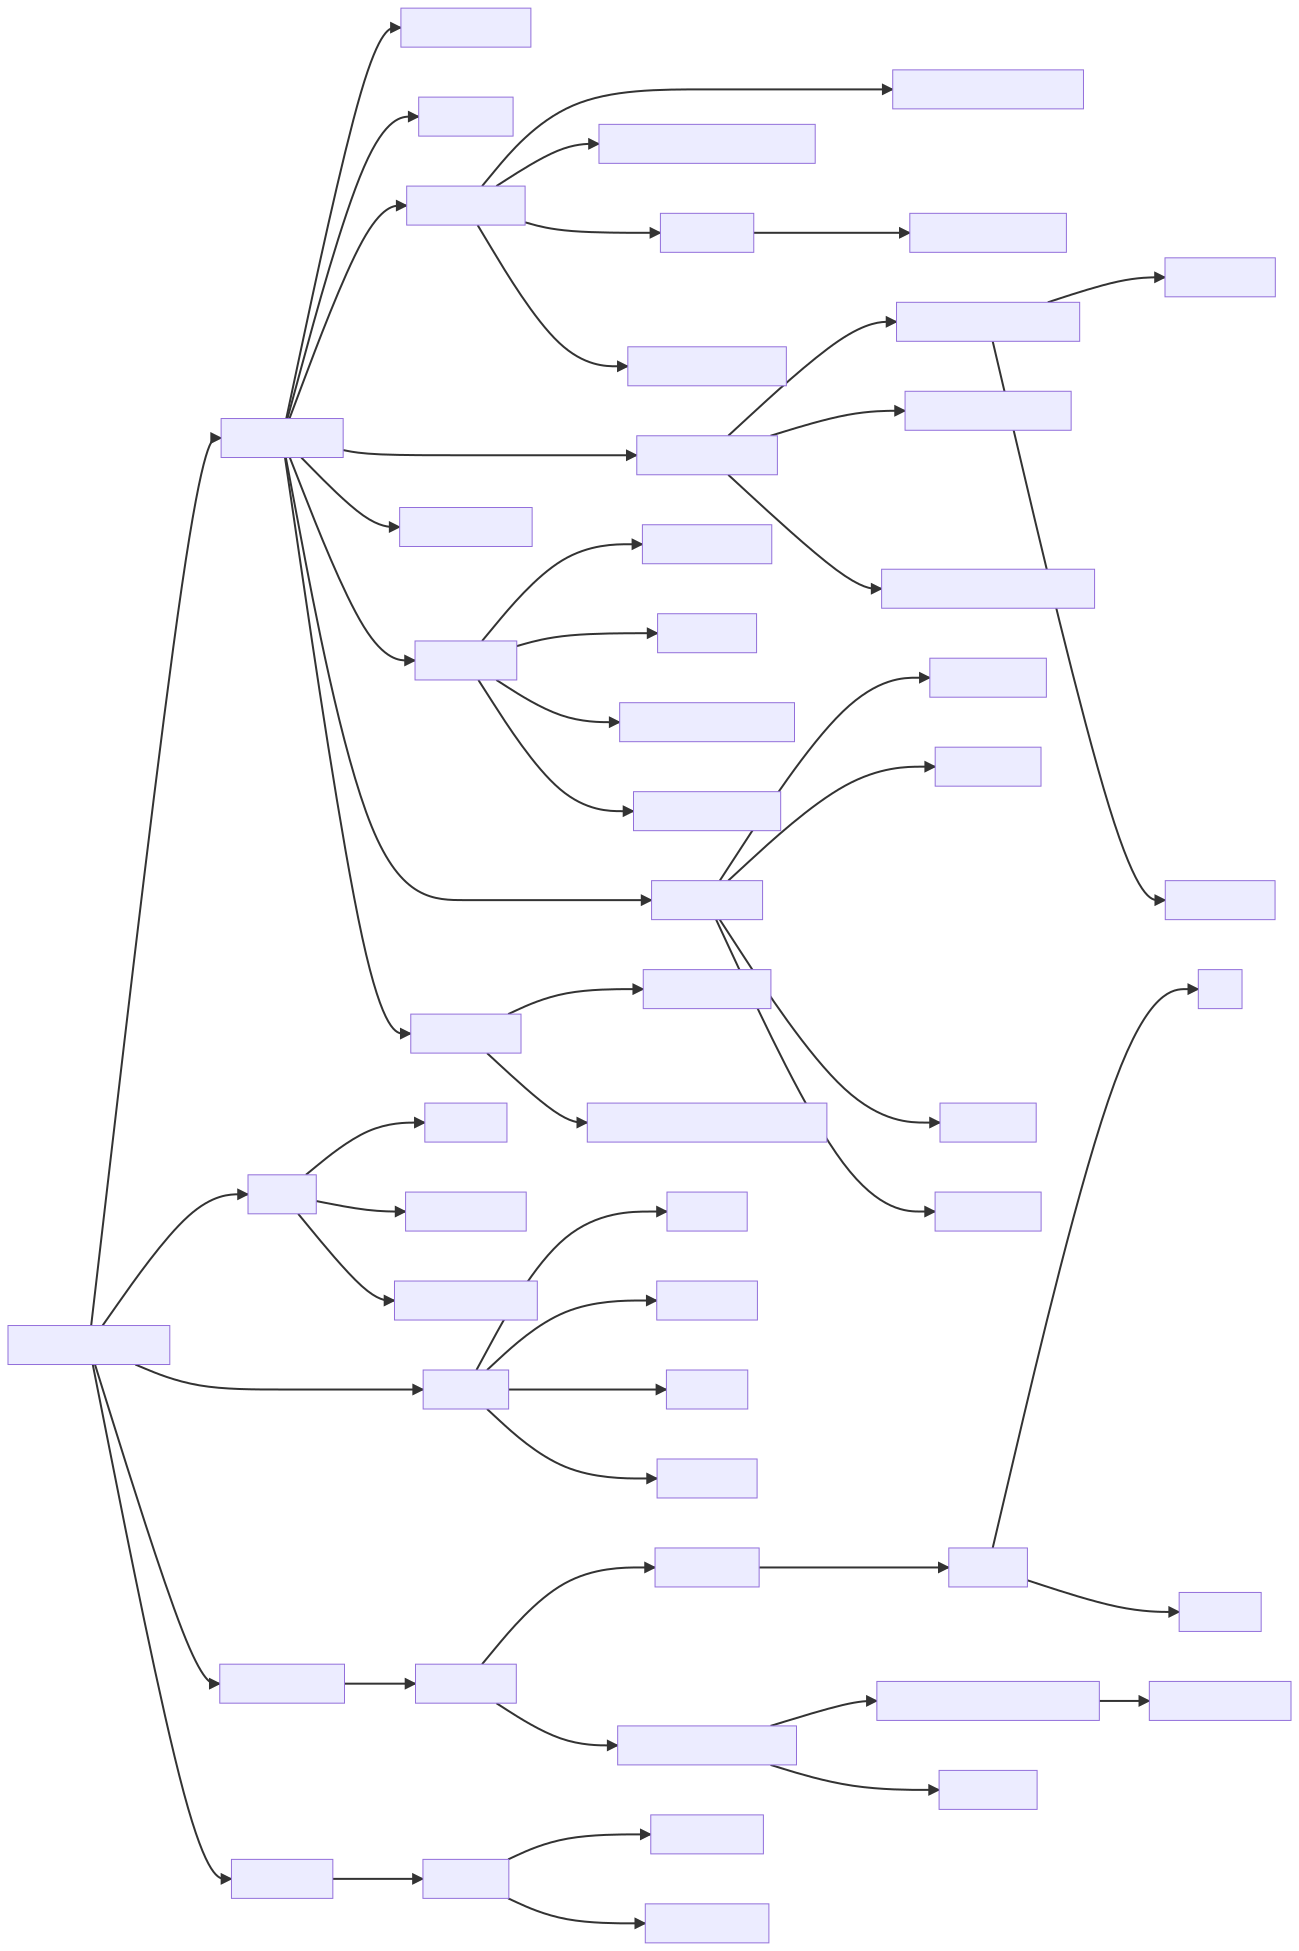
\includepdf[pages=-]{graphs/decomposition-design.pdf}

\subsection{NavigationView}
\label{sec:NavigationViewDesign}

\includegraphics[width=\textwidth, height=\textheight, keepaspectratio]{NavigationView-design}

The NavigationView provides a global menu for the user to navigate between different pages in the software. There are six tabs in the NavigationView, ``Home'', ``Problems'', ``Assignments'', ``Playground'', ``Account'', ``Settings''. By clicking on a different tab, the mainframe will display the corresponding page. The currently selected tab will be highlighted.

\subsubsection{Usability feature}

The entire NavigationView is a usability feature. Users can always look it up by clicking the top left button. They will be able to know where they are and navigate to other pages with one click, which makes the program easier to use.

\subsubsection{Validation}

There are only buttons in the NavigationView for the user to click, so only valid actions can be taken, no further data validation is required.

\subsection{HomePage}
\label{sec:HomePageDesign}

\includegraphics[width=\textwidth, height=\textheight, keepaspectratio]{HomePage-design}

The HomePage is the first page that gets displayed to the user. On the top of the HomePage, there will be a beautiful background image under the `Algorithm Dynamics' title. On the bottom, there are 10 useful buttons link to different functions.

\subsubsection{Usability feature}

The `Random' button starts a random problem for the user. The `Import' button calls the system file explorer for the user to import problems, problem lists, or assignments. The `Playground', `Problems', `Assignments' and `Account' button links the user to the corresponding page. The three buttons at the end link to three useful websites, when users click the button, the default web browser will be called and directed to these websites, which makes it easy for the user to look up specifications and revise content. All the useful functions of the software are grouped on the HomePage, which makes them easily accessible and makes the software easy to use.

\subsubsection{Validation}

There are only buttons in the HomePage for the user to click, so only valid actions can be taken, no further data validation is required.

\subsubsection{Stakeholder feedback}
\label{subsubsec:homepage stakeholder feedback}

Timofei thinks putting the links on the same page makes it messy. He thinks those websites and resources can be easily found on the Internet, so there is no need to put extra links on the HomePage.

PCloud points out that the icon grid needs to be responsive, so when he uses the software on a small screen, all buttons should still be displayed properly.

Mr Grimwood says it will be great if some greeting messages with recommendations can be displayed, such as ``You have 6 assignments to do this week.'' or ``You did pretty bad on data structures problems last time, maybe try this problem list to help you revise better.''

\subsubsection{Response}

Timofei has a good point here, and I decide to remove these links. The UI will be responsive to different window sizes, and this will be tested.

The greeting message and recommendations is a great idea. I will add an additional row below the image to display the greeting and recommendations.

\includegraphics[width=\textwidth, height=\textheight, keepaspectratio]{HomePage-Updated-design}

This is the redesigned HomePage. It adds greeting messages and recommendations. It has a responsive grid and a scroller is displayed when the item does not fit in one page. The useless links are removed.

\subsection{ProblemsPage}
\label{sec:ProblemsPageDesign}


\includegraphics[width=\textwidth, height=\textheight, keepaspectratio]{ProblemsPage-design}

The ProblemsPage displays all problems in the database. The user can search, create, edit, delete, import, export or start working on one or multiple problems on this page.

\subsubsection{Usability feature}

The user can apply the selection condition by either selecting different fields in the dropdown boxes or directly typing into the search box. A scrollable list of problems that match the conditions will be shown below with detailed information. The user can start working on a problem by clicking the start button on the right. They can also right-click the problem to call a context menu that includes more actions for them to delete, edit or export the problem. By clicking the select button on the top, the user can select multiple problems at once and apply the same action to them at once. By clicking the Add button on the top right, a context menu will be displayed, allowing the user to create or import new problems or problem lists. When the user is typing into the search box, a flyout will display matching results to save typing. I will implement an advanced searching algorithm to improve the quality of the search results, and I will explain the algorithm in the \hyperref[sec:algorithm design]{algorithm design section}.

\subsubsection{Validation}

Most components on this page are still buttons, users can only click them and no invalid data can be input. The search box is where the user can input some text only. A flyout will be displayed to promote the user to click the button instead of inputting data themselves. Also, a length check will be applied. The user can only enter a maximum of 32 characters so they cannot crash the search box or the searching algorithm. Instead of passing the search keywords directly to the database, a custom searching algorithm will be used to search and sanitise the search keyword, which prevents SQL injection and provide a better searching experience.

\subsection{CodingPage}
\label{sec:CodingPageDesign}

\includegraphics[width=\textwidth, height=\textheight, keepaspectratio]{CodingPage-design}

The CodingPage is where the user works on a programming problem. It contains a question panel, a code editor and an IO panel.

\subsubsection{Usability feature}

The question is displayed on the left and a code editor will be displayed on the top right. The input, output and error messages will be displayed on the button right, the user can switch between them by clicking the corresponding tab. On the bottom, the user can select programming language using a dropdown menu, run code by clicking the run code button and submit their code for judging by clicking the submit button. The status field shows the status of the judger and 3 navigation buttons on the button right to make it easy to navigate between different problems. There is a progress bar between the IO panel and the navigation buttons, it displays the judging progress.

The code editor will support line numbers, basic syntax highlighting and keyboard shortcuts to make it easy to use.

\subsubsection{Validaton}

Again, most of the components on the page are either read-only (such as the question section) or buttons. The code editor is the only place for the user to input text, and the text inside will be validated by the compiler or the interpreter of the selected programming language. However, the IO panel requires further validation. To prevent the user from printing out a huge amount of data which might result in poor performance, the IO panel will perform a length check and only display the first 2048 characters of the output.

\subsection{AssignmentsPage}
\label{sec:AssignmentsPageDesign}

\includegraphics[width=\textwidth, height=\textheight, keepaspectratio]{AssignmentsPage-design}

The AssignmentsPage is where the user interacts with the assignments. For students, they can work on their assignments; for teachers, they can create and mark assignments.

\subsubsection{Usability feature}

The user can switch between different tabs by clicking the navigation bar at the top. They can enter the detailed view of an assignment by clicking one assignment. A dropdown button is placed on the top right for the user to create or import a new assignment. All assignments will be displayed in a list with their due date.

\subsubsection{Validation}

There are only buttons for the user to click, so only valid actions can be taken, no further data validation is required.

\includegraphics[width=\textwidth, height=\textheight, keepaspectratio]{AssignmentsStudentDetailsPage-design}

This is the assignment details page for students, which gets displayed when a student clicks on an assignment.

\subsubsection{Usability feature}

The descriptions and due date of the assignment are displayed on the top left. A list of problems is displayed below where the user can see their status and start working on one by clicking it. When the user clicks the start button, he will be navigated to the CodingPage and the problems will be loaded. When he finishes all problems, he can click the submit button to either submit it through API or export it to a file to send to the teacher for marking.

\subsubsection{Validation}

There are only buttons for the user to click, so only valid actions can be taken, no further data validation is required.

\includegraphics[width=\textwidth, height=\textheight, keepaspectratio]{AssignmentsTeacherDetailsPage-design}

This is the assignment details page for teachers, which gets displayed when a teacher clicks on an assignment.

\subsubsection{Usability feature}

The teacher can click the Import Submissions button to import students' submissions or click the edit button to edit the assignment, or the export button to distribute the assignment. All student submissions and their status will be listed on the right, the teacher can click the mark button to mark all of them automatically and click the student submission to see the code details in the CodeingPage.

After marking, the teacher can click the export results button to export all student's marks into a CSV file for further data analysis.

\subsubsection{Validation}

There are only buttons for the user to click, so only valid actions can be taken, no further data validation is required.

\subsection{PlaygroundPage}
\label{sec:PlaygroundPageDesign}

\includegraphics[width=\textwidth, height=\textheight, keepaspectratio]{PlaygroundPage-design}

The PlaygroundPage is a free space for the user to run any code quickly. It is essentially the same page as the CodingPage but without a coding problem. The interface is slightly changed with a larger code editor and a separate IO panel for a better user experience.

\subsection{AccountPage}
\label{sec:AccountPageDesign}

\includegraphics[width=\textwidth, height=\textheight, keepaspectratio]{AccountPage-design}

The AccountPage is used to manage the current user and display user statistics.

\subsubsection{Usability feature}

If the user has login into his Microsoft account, the avatar, username, email and role will be managed by his Microsoft Account, the edit button will navigate to the Microsoft account website, and the login button will be replaced with a logout button. If the user has a login locally, he can edit his information by clicking the edit button and log in to Microsoft account by clicking the login button.

Some interesting statistics will be displayed on the button.

\subsubsection{Validation}

When the user edits his local identity, the user name will not be allowed to exceed 32 characters, and a format check will be applied to the email address.

\subsubsection{Stakeholder feedback}
\label{subsubsec:accountpage stakeholder feedback}

Timofei thinks there can be more interesting statistics, such as favourite variable names, and the total time spends in the software.

Mr Grimwood suggests that ``topic needs more revision'' can be added to the statistics.

\subsubsection{Response}
It may be too difficult to implement such statistics but this is an interesting idea. This feature is put in the backlog and will not be implemented for now.

``Topic needs more revision'' will be put as a recommendation, on the HomePage instead, which will make it more useful.

\subsection{SettingsPage}
\label{sec:SettingsPageDesign}

\includegraphics[width=\textwidth, height=\textheight, keepaspectratio]{SettingsPage-design}

The SettingsPage is where the user adjusts software settings.

\subsubsection{Usability feature}

The user can adjust the colour theme of the software to use a light theme, dark theme or system default theme. The user can also change the run code time limit, memory limit and programming language profiles in the SettingsPage.

\subsubsection{Validation}

Radio buttons are used for colour theme selection so it is impossible to enter any invalid data. A number box is used for the time limit and memory limit settings so only positive integers can be input. A dropdown list is used for the programming language setting so only valid input is accepted.

\subsubsection{Stakeholder feedback}
\label{subsubsec:settingspage stakeholder feedback}

Timofei likes the idea of being able to switch between a light theme and a dark theme. He thinks it will be better if users are allowed to create their custom themes. He also suggests that allowing the user to change the font size manually may help a lot.

\subsubsection{Response}

Extra themes take too much time to design, but it is an interesting idea. The font size is managed by the system and it is not very easy to change. Both ideas are great, they are put into the backlog and will not be implemented right away.

\subsection{CreateNewProblemPage}
\label{sec:CreateNewProblemPageDesign}

\includegraphics[width=\textwidth, height=\textheight, keepaspectratio]{CreateNewProblemPage-design}

The CreateNewProblemPage is used to create new problems. It contains multiple text boxes for the user to input problem information.

This page will be reused for editing existing problems. The title will be altered correspondingly.

\subsubsection{Usability feature}

The Tags field will be a tokenizing text box with an auto suggestion dropdown menu to make input faster. The Difficulty field will have a dropdown list for easy selection. The Time Limit and Memory Limit fields will be number boxes. The user can add a new test case by clicking the add button and removing existing ones by clicking the delete button. If the user clicks the cancel button, a flyout will be displayed to confirm cancellation.

\subsubsection{Validation}

There are many input boxes on this page, they will all be validated. For the Problem Name field, the user can enter 32 characters at maximum. In the Tags field, the user can enter 5 tags at maximum. In the Time Limit and Memory Limit fields, the user can only enter numbers.

\subsection{CreateNewProblemListPage}
\label{sec:CreateNewProblemListPageDesign}

\includegraphics[width=\textwidth, height=\textheight, keepaspectratio]{CreateNewProblemListPage-design}

The CreateNewProblemListPage is used to create a new problem list. It contains multiple text boxes for the user to input problem list information.

The page will be reused for editing existing problem lists. The title will be altered correspondingly.

\subsubsection{Usability feature}

There will be an autosuggest box for the user to search for problems and add them to the list. There is an export and a save button at the button for the user to export or save the problem list. If the user clicks the cancel button, a flyout will be displayed to confirm cancellation. The test cases will be a scrollable list to display multiple test cases.

\subsubsection{Validation}

A similar validation is performed just like the CreateNewProblempage. For the List Name field, the user can enter 32 characters at maximum.

\subsection{CreateNewAssignmentsPage}
\label{sec:CreateNewAssignmentsPageDesign}

\includegraphics[width=\textwidth, height=\textheight, keepaspectratio]{CreateNewAssignmentsPage-design}

The CreateNewAssignmentsPage is used to create new assignments. It contains multiple text boxes for the user to input assignment data.

The page will be reused for editing existing assignments as well. The title will be altered correspondingly.

\subsubsection{Usability feature}

The due date will be a DateTime picker, a visual calendar will be displayed for the user to pick a due date. An autosuggest search box will be placed for the user to search for problems easily.

\subsubsection{Validation}

The DateTime picker will prevent invalid dates from being input, the name field will have a maximum of 32 characters limit.

\subsection{Judger module}

The Judger module will handle all the judging and marking tasks. It takes in a \code{Submission}, compile and execute the user's code, judges whether it gives the correct output.

The Judger will take a few seconds to judge each \code{Submission}, while it is judging, the other parts of the software need to keep working on their tasks. So I use concurrent processing to let the Judger run parallel with the main program.

When judging a single \code{TestCase}, the Judger will first start the compiler in a new process to compile the user's code. The Judger redirects the output of the compiler to an internal string variable to store all outputs. When the compiler finishes compiling, an interrupt is triggered and the Judger will be notified that the compilation has been done. It will check the compiler's exit code and its output, if there are any compilation errors, they will be reported back. Otherwise, the Judger will run the compiled executable, and feed the input to its \code{stdin} and redirects all \code{stdout} and \code{stderr} to internal string variables. On top of that, the Judger will start a countdown timer in a different process to track the time. When the countdown reaches zero, an interrupt will be sent to the Judger and it will terminate the user's code and report a time limit exceed error, or if the user's code finishes first, then its output will be compared with the expected output, the result and all statistics will then be reported.

A problem may contain multiple test cases, so all test cases will be first pushed into a judging queue, and the judger will judge them one by one.

Similarly, an assignment may contain multiple problems, all problems will be first pushed into a problem queue, and each problem will be processed one by one.

The detailed judging algorithm will be explained later in the 
\hyperref[sec:algorithm design]{algorithm design section}.

\subsection{Database module}

Because this software will store many complex relational data, a relational database is needed to store all the data. Since the software runs locally, and every user will have different data, instead of a central SQL Server, a local SQL Database engine is required.

I choose to use SQLite to power this software. It is a small, self-contained, high-reliability, full-featured SQL Database engine, which will be enough to handle all the data storing and querying requests.

The SQLite database has some limitations. It only supports five data types. \code{TEXT}, \code{INTEGER}, \code{NULL}, \code{REAL} and \code{BLOB}. So other data types such as \code{DateTime} and \code{Guid} will need to be converted before storing.

I choose to use Microsoft.Data.SQLite for the database interface, which allows me to send SQL requests to the database, handle errors and provide safety features to prevent SQL injection. Details about the design of the database and queries will be described in the \hyperref[subsec:database design]{Database design section}.

\subsection{API module}

The API module will allow the user to log in to their Microsoft Education account, and interact with the Education Assignment function. Users will be able to create and manage assignments using education assignments APIs provided by Microsoft.

When the user clicks the login button in the SettingsPage, the API module will handle the login requests. When a logged-in user opens the AssignmentsPage, the API module will fetch all assignments. The API module will also allow the teachers to distribute assignments directly through API calls and the students to hand in submissions without any kind of exporting.

The API module will be implemented at the end after all local functions are working correctly. The corresponding API calls and endpoints will be discussed later.

\subsection{Stakeholder feedback}

I conduct an interview with each stakeholder after designing all the user interface elements. The statkeholders are generally very satisfying with the design. Suggestions are mainly about the \hyperref[subsubsec:homepage stakeholder feedback]{HomePage design} and the \hyperref[subsubsec:accountpage stakeholder feedback]{AccountPage design}, I have recorded their suggestions and my responses in those sections.

\section{Algorithm design}
\label{sec:algorithm design}

\subsection{Searchbox searching algorithm}

This algorithm will be used to power all the search boxes in the software. It will be packed into a function, taking in a list of items and the searching keyword input by the user, returning a list of results. To make the software easy to use, instead of simply using a linear search and returning all matching results, the algorithm will perform some fuzzy searching, so even the word is not typed in completely, matching results will be returned.

\begin{minted}{text}
function search(sourceList, keyword)
    // Create an empty list to store the results
    resultList = new List<string>()
    // Split the keyword into pieces by space
    splitKeyword = keyword.ToLower().Split(' ')
    // Compare each piece of keyword with the sourceList
    // Add the matching result into resultList
    for i=0 to sourceList.Length - 1
        for j=0 to splitKeyword.Length - 1
        sourceKey = sourceList[i].ToLower()
            if sourceKey.Contains(splitKeyword[j]) then
                resultList.Add(sourceList[i])
            endif
        next j
    next i

    // If no result is found,
    // add an "not found" notice to the resultList
    if resultList.Length == 0 then
          resultList.Add("No results found")
    endif
endfunction
\end{minted}

In this algorithm, I first create an empty list to store the result. Then I split the keyword into a list by space. So the keyword ``A Long Problem Name'' will be splitted into \code{["A", "Long", "Problem", "Name"]}.

Next, I use two nested loops to perform a linear search on each keyword. I choose to use the linear search here because the list is not sorted, so only it will work. The overall time complexity here is $O(nm)$ where $n$ is the length of the \code{sourceList} and $m$ is the length of \code{splitKeyword}. This is not very fast, but in real-world use cases, both $n$ and $m$ will be very small (less than 1000), so this algorithm will be fast enough to handle most of the cases. The increase in complexity brings a better searching experience. In this way, the algorithm will be able to match keywords like ``prob'' to result in ``A Long Problem List'', while normal linear search will not be able to do this.

In the end, if no item is found, a not found notice is added to the list, which will be displayed to the user.

\subsection{Judger RunCode algorithm}

This algorithm is designed for the Judger to run a piece of code, pass input to the code and receive all the output and error. This is the basic function of the Judger and further judging will all base on this algorithm.

Before anything can run, the Judger will need to first write the user's code to a source code file. And before it can do that, it needs to know where it should write to. I will create three private variables \code{_SourceCodeFilePath}, \code{_SourceCodeFolderPath} and \code{_ExecutableFilePath} to store the file paths for the source code file and the executable file. I use the idea of encapsulation here so these variables can only be set by the public method \code{SetSourceCodeFilePath}, so they will not be modified unexpectedly.

\begin{minted}{text}
partial class Judger
    private _SourceCodeFilePath
    private _SourceCodeFolderPath
    private _ExecutableFilePath

    public procedure SetSourceCodeFilePath(FolderPath, FileName)
        _SourceCodeFolderPath = FolderPath
        _SourceCodeFilePath = FolderPath + FileName + ".txt"
        _ExecutableFilePath = FolderPath + FilePath + ".exe"
    endprocedure
endclass
\end{minted}

For compiling programming languages such as C, C++ and Java, the source code needs to be compiled before running. So I need to add a \code{Compile} function to support these programming languages. The compile task needs to be run concurrently in a different process so the main UI can stay responsive. So instead of monitoring the compiler all the time, I will bind two event handlers to the compile process, to process its output data and error data. Those data will then be stored in two private string variables for later use.

\begin{minted}{text}
partial class Judger
    private _CompilationOutput
    private _CompilationError

    private procedure CompileProcess_ErrorDataReceived(sender, e)
        // Validate the data before storing
        if string.IsNullOrEmpty(e.Data) == False then
            _CompilationError += e.Data + '\n'
        endif
    endprocedure

    private procedure CompileProcess_OutputDataReceived(sender, e)
        // Validate the data before storing
        if string.IsNullOrEmpty(e.Data) == False then
            _CompilationOutput += e.Data + '\n
        endif
    endprocedure
endclass
\end{minted}

Now, it is ready to run the compiler. Before it can start compiling, the old outputs need to be cleaned. I design two magic variables in the language configurations allowing more flexible arguments, these magic variables need to be pre-processed before compiling. A process start info needs to be created to let the Judger know how to start the new process. After binding the event handlers, the compiler can start running.

\begin{minted}{text}
partial class Judger
    private function Compile()
        // Clear the old data
        _CompilationOutput = ""
        _CompilationError = ""

        // Pre-process language compile command and arguments
        string fileName = language.CompileCommand.Replace("{SourceCodeFilePath}", _SourceCodeFilePath).Replace("{ExecutableFilePath}", _ExecutableFilePath)
        string arguments = language.CompileArguments.Replace("{SourceCodeFilePath}", _SourceCodeFilePath).Replace("{ExecutableFilePath}", _ExecutableFilePath)
        
        // Create a new process start info
        ProcessStartInfo StartInfo = new ProcessStartInfo
        (
            FileName: fileName,
            Arguments: arguments,
            UseShellExecute: false,
            CreateNoWindow: true,
            RedirectStandardOutput: true,
            RedirectStandardError: true,
        )
        
        // Create a new compile process
        Process CompileProcess = new Process(StartInfo)
        
        // Bind event handlers to the compile process
        CompileProcess.OutputDataReceived += new DataReceivedEventHandler(CompileProcess_OutputDataReceived)
        CompileProcess.ErrorDataReceived += new DataReceivedEventHandler(CompileProcess_ErrorDataReceived)
        
        // Start the compile process
        CompileProcess.Start()
        CompileProcess.BeginOutputReadLine()
        CompileProcess.BeginErrorReadLine()
        CompileProcess.WaitForExitAsync()

        // Return the exit code
        return CompileProcess.ExitCode
    endfunction
endclass
\end{minted}

In the end, an integer exit code will be returned. If the exit code is zero, the Judger will know that the compilation is successful. If it is something else, then the Judger will need to report a compile error with detailed data from \code{_CompilationError}. 

If the user's code is compiled successfully or it does not need to be compiled, the \code{Execute} function is called to run the code or the executable, pass the input to the process and get its output. The \code{Execute} function will also need to kill the running process if it runs too long. So I will use a custom enumeration type \code{StatusCode} to manage the process' status.

\begin{minted}{text}
enum StatusCode
    PENDING,
    RUNNING,
    FINISHED,
    TIME_LIMIT_EXCEEDED,
    MEMORY_LIMIT_EXCEED
endenum

partial class Judger
    private _StatusCode
endclass
\end{minted}

\code{StatusCode} has five possible values, \code{PENDING} is set when the code is waiting to be run. When it starts executing, the status code will be set to \code{RUNNING}. If it finishes in time, its status will be set to \code{FINISHED}. If it exceeds the time limit, the process will be killed by the Judger and a \code{TLE} will be recorded. If it exceeds the memory limit, the process will be killed by the Judger and a \code{MLE} will be recorded.

Similarly, I will use event handlers to record all the outputs from the user's code. I add a third handler to process the exit event, which will determine the \code{_StatusCode} mentioned above.

\begin{minted}{text}
partial class Judger
    private _StandardOutput
    private _StandardError

    private procedure ExecuteProcess_Exited(sender, e)
        // Only successfully finished when the status code is not TLE or MLE
        if _StatusCode != StatusCode.TIME_LIMIT_EXCEEDED and _StatusCode != StatusCode.MEMORY_LIMIT_EXCEED then
            _StatusCode = StatusCode.FINISHED
        endif
    endprocedure

    private procedure ExecuteProcess_OutputDataReceived(sender, e)
        // Validate the data before storing
        if string.IsNullOrEmpty(e.Data) == False then
            _StandardOutput += e.Data + '\n'
        endif
    endprocedure

    private procedure ExecuteProcess_ErrorDataReceived(sender, e)
        // Validate the data before storing
        if string.IsNullOrEmpty(e.Data) == False then
            _StandardError += e.Data + '\n'
        endif
    endprocedure
endclass
\end{minted}

The \code{Execute} function has a similar design with the \code{Compile} function. It configures all the running information and event handlers as usual. However, this time I add two extra processes running concurrently with the execution process. The first one is a timer, which countdown the time limit. When the timer counts to zero, it checks whether the execute process is still running, if it does, then the execution process will be killed and a \code{TLE} will be reported. The second one is a memory monitor, which checks the peak memory usage of the execution process every 10 milliseconds. If the memory usage is larger than the memory limit, then the execution process will be killed and a \code{MLE} will be reported.

\begin{minted}{text}
partial class Judger
    private _WorkingSet64;
    private function Execute(Input, Language, TimeLimit, MemoryLimit)
        // Clear the old data
        _StandardOutput = ""
        _StandardInput = ""
        _WorkingSet64 = 0

        // Initialize status code
        _StatusCode = StatusCode.PENDING

        // Pre-process language run command and arguments
        string fileName = Language.RunCommand.Replace("{SourceCodeFilePath}", _SourceCodeFilePath).Replace("{ExecutableFilePath}", _ExecutableFilePath)
        string arguments = Language.RunArguments.Replace("{SourceCodeFilePath}", _SourceCodeFilePath).Replace("{ExecutableFilePath}", _ExecutableFilePath)

        // Create a new process start info
        ProcessStartInfo StartInfo = new ProcessStartInfo
        (
            FileName: fileName,
            Arguments: arguments,
            UseShellExecute: false,
            CreateNoWindow: true,
            RedirectStandardInput: true,
            RedirectStandardOutput: true,
            RedirectStandardError: true,
        )

        // Create a new execute process
        Process ExecuteProcess = new ExecuteProcess(StartInfo)

        // Bind event handlers to the compile process
        ExecuteProcess.OutputDataReceived += new DataReceivedEventHandler(ExecuteProcess_OutputDataReceived)
        ExecuteProcess.ErrorDataReceived += new DataReceivedEventHandler(ExecuteProcess_ErrorDataReceived)
        ExecuteProcess.Exited += new EventHandler(ExecuteProcess_Exited)
        
        // Start the execute process
        ExecuteProcess.Start()
        ExecuteProcess.BeginOutputReadLine()
        ExecuteProcess.BeginErrorReadLine()
        ExecuteProcess.StandardInput.WriteLine(Input);

        // Set the status code to Running
        _StatusCode = StatusCode.RUNNING
        
       // Start the timer
        Timer timer = new Timer(() => 
        {
            // If the user's code is still running 
            // when the timer has finished
            // Kill the user's code and record a TLE
            if ExecuteProcess.HasExited == false then
                ExecuteProcess.Kill()
                _StatusCode = StatusCode.TIME_LIMIT_EXCEEDED
            endif
        }, null, TimeLimit, Timeout.Infinite)

        // Start the memory monitor
        Thread MemoryMonitor = new Thread(() =>
        {
            while ExecuteProcess.HasExited == false
                ExecuteProcess.Refresh()
                _WorkingSet64 = ExecuteProcess.PeakWorkingSet64
                if _WorkingSet64 > MemoryLimit then
                    ExecuteProcess.Kill()
                    _StatusCode = StatusCode.MEMORY_LIMIT_EXCEEDED
                endif
            endwhile
        });
        MemoryMonitor.Start()

        // Wait the process to finish
        ExecuteProcess.WaitForExitAsync()

        // Return the exit code
        return ExecuteProcess.ExitCode
    endfunction
endclass
\end{minted}

Now I have everything I need to build the \code{RunCode} function. It takes in the user's code, input data, language configuration, time limit and memory limit, outputs a \code{RunCodeResult} containing all the running information. I also need to set up a stopwatch to measure how long the code has been executed, unlike the timer before, this stopwatch only provides data for statistics records. In the end, the \code{RunCode} function will handle some basic errors, it will judge whether the user's code run, but it will not judge whether the user's code provides the correct output. The \code{RunCode} algorithm only runs the code and further judging will be handed over to other algorithms.

\begin{minted}{text}
partial class Judger
    public function RunCode(UserCode, Input, Language, TimeLimit, MemoryLimit)
        // Create a new TestCaseResult
        RunCodeResult result = new RunCodeResult()

        // Write the source code to file
        sourceCodeFile = openWrite(_SourceCodeFilePath)
        sourceCodeFile.write(UserCode)
        sourceCodeFile.close()

        // Compile if needed
        if Language.NeedCompile then
            // Compile and record the exit code
            exitCode = Compile(Language)

            // If compile failed then return a COMPILE_ERROR
            if exitCode != 0 then
                result.StandardOutput = _CompilationOutput
                result.StandardError = _CompilationError
                result.ResultCode = ResultCode.COMPILE_ERROR
                return result
            endif
        endif

        // Set up a Stopwatch to record the running time
        Stopwatch watch = new Stopwatch()
        watch.Start()

        // Execute the code
        exitCode = Execute(Input, Language, TimeLimit)

        watch.Stop()

        // Store the stats to the result
        result.StandardOutput = _StandardOutput
        result.StandardError = _StandardError
        result.CPUTime = watch.ElapsedMilliseconds

        // If time limit exceed, return TLE
        if _StatusCode == StatusCode.TIME_LIMIT_EXCEEDED then
            result.ResultCode = ResultCode.TIME_LIMIT_EXCEEDED
            return result
        endif

        // If memory limit exceed, return MLE
        if _StatusCode == StatusCode.MEMORY_LIMIT_EXCEEDED then
            result.ResultCode = ResultCode.MEMORY_LIMIT_EXCEEDED
            return result
        endif

        // If receive a error or exit code is not zero
        // Return a runtime error
        if string.IsNullOrEmpty(result.StandardError) == False or exitCode != 0 then
            result.ResultCode = ResultCode.RUNTIME_ERROR
            return result
        endif

        // Otherwise, return success
        result.ResultCode = ResultCode.SUCCESS
        return result
    endfunction
endclass
\end{minted}

\subsection{Judger Judge TestCase algorithm}

This algorithm is designed to allow the Judger to judge a test case. On top of the \code{RunCode} function, this algorithm compare the user's output with the expected output, so it can judge whether the user's code works correctly. The \code{JudgeTestCase} function returns a \code{TestCaseResult} containing more information.

\begin{minted}{text}
partial class Judger
    public function JudgeTestCase(UserCode, TestCase, Language, TimeLimit)
        // Run the code with RunCode and get the result
        TestCaseResult result = (TestCaseResult)RunCode(UserCode, TestCase.Input, Language, TimeLimit)
        result.TestCase = TestCase

        // If the code is executed successfully
        // Judge whether its output matches the expected output
        if result.ResultCode == ResultCode.SUCCESS then

            // Trim the trailing spaces before comparing
            userOutput = result.StandardOutput.Trim()
            expectedOutput = TestCase.Output.Trim()

            // If they are not matched
            // Report wrong answer
            if userOutput != expectedOutput then
                result.ResultCode = ResultCode.WRONG_ANSWER
            endif
        endif
        return result
    endfunction
endclass  
\end{minted}

\subsection{Judger Judge Problem algorithm}

This algorithm is designed to judge a submission. I set up a judging queue and push all test cases into the queue. Then I take them out and judge them one by one. A queue is suitable for this use case because I want the first test case entered to be judged first. A submission result will be returned at the end.

\begin{minted}{text}
partial class Judger
    public function JudgeProblem(Submission)
        // Create the submission result
        SubmissionResult result = new SubmissionResult()
        result.Submission = Submission

        // Create the judging queue
        Queue JudgeQueue = new Queue(Submission.Problem.TestCases)

        // Keep judging until the queue is empty
        while len(JudgeQueue) > 0
            Code = Submission.Code
            TestCase = JudgeQueue.Dequeue()
            Language = Submission.Language
            TimeLimit = Submission.Problem.TimeLimit
            MemoryLimit = Submission.Problem.MemoryLimit
            TestCaseResult = JudgeTestCase(Code, TestCase, Language, TimeLimit, MemoryLimit)
            result.Add(TestCaseResult)
        endwhile
        return result
    endfunction
endclass
\end{minted}

\subsection{Judger Judge Assignment algorithm}

This algorithm is designed to judge an assignment submission. I set up a judging queue and push all problems into the queue. Then I take them out and judge them one by one. A queue is suitable for this use case because I want the first problem entered to be judged first. An assignment submission result will be returned at the end.

\begin{minted}{text}
partial class Judger
    public function JudgeAssignment(AssignmentSubmission)
        // Create the assignment submission result
        AssignmentSubmissionResult result = new AssignmentSubmissionResult()
        result.AssignmentSubmission = AssignmentSubmission

        // Create the judging queue
        Queue JudgeQueue = new Queue(AssignmentSubmission.Submissions)

        // Keep judging until the queue is empty
        while len(JudgeQueue) > 0
            Submission = JudgeQueue.Dequeue()
            SubmissionResult = JudgeProblem(Submission)
            result.Add(SubmissionResult)
        endwhile
        return result
    endfunction
endclass
\end{minted}

\section{Data structure design}

\subsection{Class design}

I am taking an object-oriented approach to the design of the software. This is the class diagram for all classes with their attributes and methods.

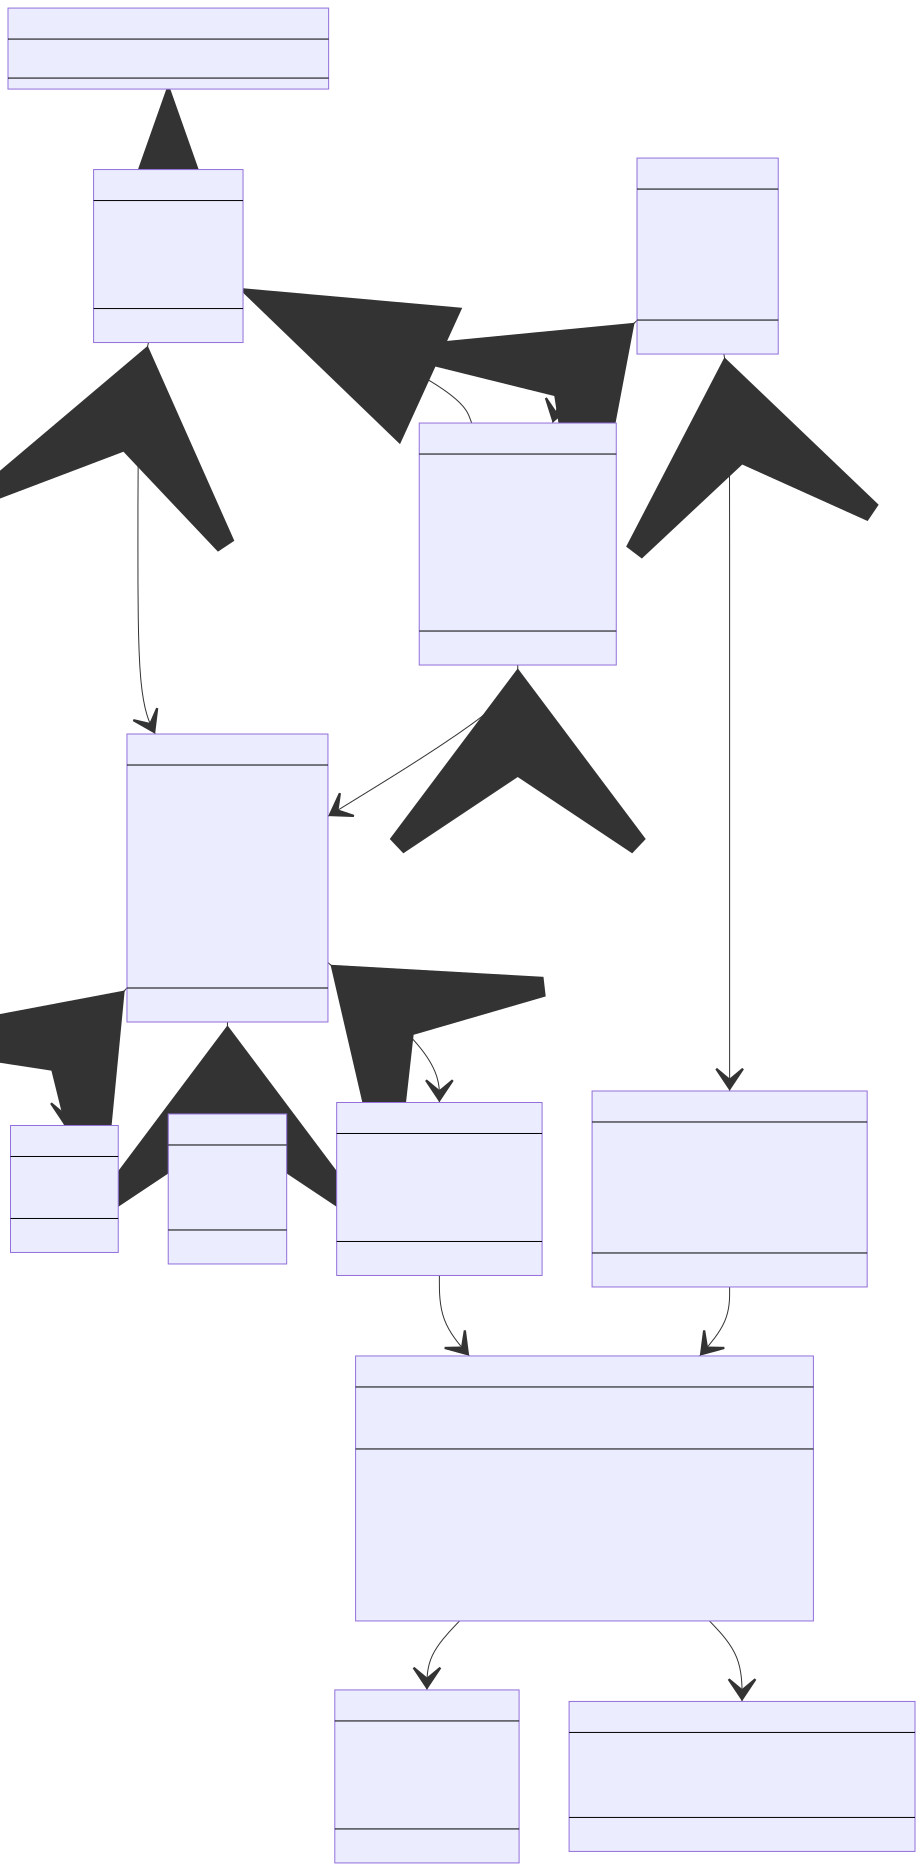
\includegraphics[width=\textwidth, height=\textheight, keepaspectratio]{classDiagram}

\subsubsection{User}

\code{User} is an object used to represent the current user. Its data will be attached to each \code{Submission}, \code{Assignment} and \code{AssignmentSubmission}, so the user can track identities and manage the data easily. Users will be asked to enter this information when they first open the software, an instance of \code{User} will be created and stored in the database.

\begin{tabulary}{\textwidth}{|l|l|L|}
    \hline
    Variable & Data type & Justification \\
    \hline
    \code{Uid} & \code{Guid} & The \code{User} uses a \code{Guid} value for its \code{Uid} instead of a normal \code{int} value to ensure the \code{Uid} is unique globally. Every user will have a unique \code{Uid}. \\
    \hline
    \code{Name} & \code{string} & \code{Name} stores the user's name. \\
    \hline
    \code{Email} & \code{string} & \code{Email} stores the user's Email address. \\
    \hline
    \code{Role} & \code{enum Role} & \code{Role} is a custom enumeration type which has two possible values, \code{Student} or \code{Teacher}. It is used to determine the role of the current user, and the user interface will be adjusted accordingly. I choose to use a custom enumeration type instead of some magic numbers to make the code more readable and easier to maintain. \\
    \hline
\end{tabulary}

\subsubsection{Tag}

A \code{Tag} is a label used to categorize a \code{Problem}.

\begin{tabulary}{\textwidth}{|l|l|L|}
    \hline
    Variable & Data type & Justification \\
    \hline
    \code{Id} & \code{int} & The \code{Id} is the local unique identifier for a \code{Tag}. It is used to uniquely determine a \code{Tag} in the local database. \\
    \hline
    \code{Name} & \code{string} & \code{Name} stores the name of the \code{Tag}. A \code{Name} must be unique, so data needs to be validated and two \code{Tags} with the same \code{Name} is not allowed. \\
    \hline
\end{tabulary}

\subsubsection{TestCase}

A \code{TestCase} is one set of test input and output, which will be used by the \code{Judger} to judge the user's submission.

\begin{tabulary}{\textwidth}{|l|l|L|}
    \hline
    Variable & Data type & Justification \\
    \hline
    \code{Id} & \code{int} & The \code{Id} is the local unique identifier for a \code{TestCase}. It is used to uniquely determine a \code{TestCase} in the database. \\
    \hline
    \code{Input} & \code{string} & The \code{Input} will be feed to the user's submission code by the \code{Judger}. \\
    \hline
    \code{Output} & \code{string} & \code{Output} stores the expected \code{Output} of the corresponding \code{Input}. The \code{Judger} will compare user's output with the \code{Output} to judge whether the user's code is correct. \\
    \hline
    \code{IsExample} & \code{bool} & Define whether this \code{TestCase} is an example. An example \code{TestCase} will be displayed to the user for debugging, and distribute with an \code{Assignment}. A non-example \code{TestCase} will be used to judge the solution and will not be displayed to the user or distribute with an \code{Assignment}. A boolean value is suitable to store the two-state data. \\
    \hline
\end{tabulary}

\subsubsection{Problem}

The \code{Problem} is used to store and organize the data for each programming question.

\begin{tabulary}{\textwidth}{|l|l|L|}
    \hline
    Variable & Data type & Justification \\
    \hline
    \code{Id} & \code{int} & The \code{Id} is the local unique identifier for a \code{Problem}. It is used to uniquely determine a \code{Problem} in the database. When a \code{Problem} is imported in to the database, a new \code{Id} is given. \\
    \hline
    \code{Name} & \code{string} & The \code{Name} is a string contains the name of a \code{Problem}. \\
    \hline
    \code{SourceHash} & \code{string} & This field is \code{null} for all normal \code{Problem}. It is only set for \code{Problem} which comes with an \code{Assignment}, and it is set to the hash value of the original \code{Problem}. This value will be recorded for \code{Submission}. \\
    \hline
\end{tabulary}

\begin{tabulary}{\textwidth}{|l|l|L|}
    \hline
    Variable & Data type & Justification \\
    \hline
    \code{Description} & \code{string} & The \code{Description} is a string storing the detailed description of a \code{Problem}. Markdown syntax is supported for a better user experience. \\
    \hline
    \code{Status} & \code{enum Status} & \code{Status} is an enumeration type containing 3 possible status: \code{Todo}, \code{Solved} and \code{Attempted}. This is used to collect user statistics data. I choose to use a custom enumeration type instead of some magic numbers to make the code more readable and easier to maintain. \\
    \hline
    \code{Difficulty} & \code{enum Difficulty} & \code{Difficulty} is an enumeration type containing 3 possible difficulties: \code{Easy}, \code{Medium} and \code{Hard}. This provdes a way for the user to search and select problems by their difficulties. \\
    \hline
    \code{TimeLimit} & \code{int} & \code{TimeLimit} sets the max time allowed for the user code to run in millisecond. When the running time exceed the \code{TimeLimit}, the running code will be killed and a Time Limit Exceed error will be recorded. This prevents infinite loop from using up all computing resources and rejects inefficient algorithms. \\
    \hline
    \code{MemoryLimit} & \code{int} & \code{MemoryLimit} sets the max memory allowed for the user's code to consume in bytes. When the memory usage exceed the memory limit, the running code will be killed and a Memory Limit Exceed Error will be recorded. This prevents incorrect code from using up all memory space and rejects inefficient algorithms. \\
    \hline
    \code{TestCases} & \code{List<TestCase>} & \code{TestCases} is a list containing all \code{TestCase} for the problem. A list is more appropriate than an array because it allows new \code{TestCase} to be added or remove existing ones during runtime. \\
    \hline
    \code{Tags} & \code{List<Tags>} & \code{Tags} is a list containing all \code{Tags} for a \code{Problem}. Similarly, I use a list for \code{Tags} so it can be added or removed during runtime. \\
    \hline
\end{tabulary}

\subsubsection{Language}

\code{Language} defines the compiling and running configurations for different programming languages. Language configurations are not stored in the database, instead, they are stored in the settings file, so users can add their custom configurations easily.

\begin{tabulary}{\textwidth}{|l|l|L|}
    \hline
    Variable & Data type & Justification \\
    \hline
    \code{Name} & \code{string} & \code{Name} stores the name of each programming language. The \code{Name} will be displayed in the drop down menu for the user to select their preferred programming language. \\
    \hline
    \code{NeedCompile} & \code{bool} & Some programming languages need to be compiled before running, such as C, C++ and Java. This attribute is used to tell the \code{Judger} to compile the code before executing. \\
    \hline
    \code{CompileCommand} & \code{string} & If a programming language requires compilation, this command is executed to call the compiler. \\
    \hline
    \code{CompileArguments} & \code{string} & If a programming language requires compilation, this arguments is passed to the compiler to specify file path and related compile arguments. \\
    \hline
    \code{RunCommand} & \code{string} & The \code{Judger} uses this command to run the executable or call the intrepreter. \\
    \hline
    \code{RunArguments} & \code{string} & This \code{Judger} pass this arguments to the executable or the intrepreter. \\
    \hline
\end{tabulary}

\subsubsection{Submission}

A \code{Submission} is created when the user submits a code solution to the \code{Judger}. The \code{Submission} will contain all the information including the time, the source code, the programming language selected and the corresponding \code{Problem} for the \code{Judger} to judge.

\begin{tabulary}{\textwidth}{|l|l|L|}
    \hline
    Variable & Data type & Justification \\
    \hline
    \code{Id} & \code{int} & The \code{Id} is the local unique identifier for a \code{Submission}. It is used to uniquely determine a \code{Submission} in the database. \\
    \hline
    \code{Problem} & \code{Problem} & The \code{Problem} contains the corresponding \code{Problem} of this \code{Submission}, which also contains the \code{TestCases} for the \code{Judger} to judge the \code{Submission}. Before storing a \code{Submission} into the database, this value needs to be normalized to the \code{Id} of that \code{Problem}. \\
    \hline
    \code{Code} & \code{string} & \code{Code} stores the submitted code, which will be executed and judged by the \code{Judger}. \\
    \hline
    \code{SubmittedTime} & \code{DateTime} & \code{SubmittedTime} stores the time the \code{Submission} is created. Instead of using a \code{string} or an \code{int} value, I decide to use the native data type \code{DateTime} provided by C\#, which makes it easier to process date time, and prevent any formating issues. \\
    \hline
    \code{Language} & \code{Language} & \code{Language} stores the programming language selected by the user, so the \code{Judger} knows how to run the code.\\
    \hline
    \code{Submitter} & \code{User} & \code{Submitter} stores the \code{User} who submits this \code{Submission}. This field will be normalized to the \code{User.Uid} before storing into the database. \\
    \hline
\end{tabulary}

\subsubsection{ProblemList}

A \code{ProblemList} is a list of \code{Problem}, which allows the user to share multiple \code{Problem} easily. It is also the parent of \code{Assignment} and provides basic functions for it. The \code{ProblemList} contains a \code{List<Problem>} variable, which provides all basic functions for a list, such as add, remove, sort and find, so I don't need to reinvent the wheel. I choose a list instead of an array because the number of \code{Problem} inside the list will be changed during runtime, so a list is more appropriate for my use case.

\begin{tabulary}{\textwidth}{|l|l|L|}
    \hline
    Variable & Data type & Justification \\
    \hline
    \code{Id} & \code{int} & The \code{Id} is the local unique identifier for a \code{ProblemList}. It is used to uniquely determine a \code{ProblemList} in the database. \\
    \hline
    \code{Name} & \code{string} & \code{Name} stores the name of the \code{Problem List}. \\
    \hline
    \code{Description} & \code{string} & \code{Description} stores the description of the \code{ProblemList}. \\
    \hline
    \code{Problems} & \code{List<Problem>} & \code{Problems} is a list of \code{Problem}, which supports basic functions to manipulate a list of data. \\
    \hline
\end{tabulary}

\subsubsection{Assignment}

An \code{Assignment} is a \code{ProblemList} which gets distributed to students. When an \code{Assignment} is distributed, a copy of that \code{Assignment} is created. All \code{TestCases} with \code{IsExample} set to \code{false} will be removed to prevent students from cheating. The \code{Type} of the \code{Assignment} will be set to \code{Copy} to indicate it is a distributed copy. The \code{Judger} will reject to judge a distributed \code{Assignment} and the \code{AssignmentsPage} will show the \code{Assignment} under the Assigned tab instead of the Created tab.

\code{Assignment} is inheriate from the \code{ProblemList}, so it can reuse the \code{Name} and \code{Description} attributes and all methods to manage a list of \code{Problem}. Upon that, new attributes and methods are added to make it functional.

\begin{tabulary}{\textwidth}{|l|l|L|}
    \hline
    Variable & Data type & Justification \\
    \hline
    \code{Uid} & \code{Guid} & The \code{Assignment} uses a \code{Guid} value for its \code{Uid} instead of a normal \code{int} value to ensure the \code{Uid} is unique globally. So when the user import an \code{Assignment} into their database, the \code{Uid} will not conflict with any existing values, and it will not be changed (Unlike a \code{ProblemList}, for which will be assigned a new \code{Id} when importing). The \code{Uid} will be referenced by the \code{AssignmentSubmission} so the \code{Judger} will be able to know which \code{Assignment} it is judging. \\
    \hline
    \code{DueDate} & \code{DateTime} & The \code{DueDate} stores the time for the due date of the \code{Assignment}. Instead of using a \code{string} or an \code{int} value, I decide to use the native data type \code{DateTime} provided by C\#, which makes it easier to process date time, and prevent all formating issues. \\
    \hline
    \code{Status} & \code{enum Status} & \code{Status} is an enumeration type containing 4 possible status for a source \code{Assignment}: \code{Draft}, \code{Scheduled}, \code{Published} and \code{Assigned} for the teacher to manage the lifecycle of an \code{Assignment}. For a distributed \code{Assignment}, there are 4 possible \code{Status}, \code{NotStarted}, \code{InProgress}, \code{Completed} and \code{OverDue}, which helps the student to manage the lifecycle of an \code{Assignment}. I choose to use a custom enumeration type instead of some magic numbers to make the code more readable and easier to maintain.\\
    \hline
    \code{Type} & \code{enum Type} & \code{Type} is an enumeration type containing 2 possible types, \code{Source} or \code{Copy}. It is used to manage the distribution of an \code{Assignment} as described above. \\
    \hline
    \code{Assigner} & \code{User} & \code{Assigner} stores the \code{User} who assigns the \code{Assignment}. This field will be normalized into the \code{User.Uid} before storing into the database. \\
    \hline
\end{tabulary}

\subsubsection{AssignmentSubmission}

When a student finishes an \code{Assignment}, an \code{AssignmentSubmission} is created for the \code{Judger} to judge. The \code{AssignmentSubmission} can either be exported to file and sent to the teacher, or it can be uploaded using API. The teacher imports the \code{AssignmentSubmission} or uses API to load it, and the \code{Judger} will be able to mark it and return the result.

\begin{tabulary}{\textwidth}{|l|l|L|}
    \hline
    Variable & Data type & Justification \\
    \hline
    \code{Uid} & \code{Guid} & The \code{AssignmentSubmission} uses a \code{Guid} value for its \code{Uid} instead of a normal \code{int} value to ensure the \code{Uid} is unique globally. So when teachers import an \code{AssignmentSubmission} into their database, the \code{Uid} will not conflict with any existing values, and it will not be changed. \\
    \hline
    \code{Submitter} & \code{User} & The user information is collected when exporting an \code{AssignmentSubmission}, so the teacher will be able to know who is the \code{Submitter}. This field needs to be normalized into \code{User.Uid} before storing into the database. \\
    \hline
    \code{Assignment} & \code{Assignment} & The \code{Assignment} corresponding to this \code{AssignmentSubmission} is recorded, so the \code{Judger} knows how to judge it. This field needs to be normalized into \code{Assignment.Uid} before storing into the database. \\
    \hline
    \code{Submissions} & \code{List<Submission>} & \code{Submissions} stores a list of \code{Submission}, which contains the user's \code{Submission} for each \code{Problem} assigned. \\
    \hline
    \code{Status} & \code{enum Status} & \code{Status} is an enumeration type containing 3 possible types, \code{NotJudged}, \code{Judged} and \code{Returned} for the teacher to keep track of each submission. \\
    \hline
\end{tabulary}

\subsubsection{Judger}

The \code{Judger} is a static class, only eposes 5 functions to run and judge user's code. The \code{Judger} takes a \code{Submission} as an input, and outputs a \code{SubmissionResult}. No variable is exposed. The private attributes and methods are discussed in the \hyperref[sec:algorithm design]{algorithm design section}.

\subsubsection{RunCodeResult}

\code{RunCodeResult} stores the judging result for a piece of code. It does not store the information about whether the output is correct, it only stores the runtime statistics and whether the code has been compiled and executed correctly. This result will not be stored in the database, so there is no \code{Id} attribute.

\begin{tabulary}{\textwidth}{|l|l|L|}
    \hline
    Variable & Data type & Justification \\
    \hline
    \code{StandardOutput} & \code{string} & \code{StandardOutput} stores the content output by the user's code. \\
    \hline
    \code{StandardError} & \code{string} & \code{StandardError} stores the error messages received (if any) when executing the user's code. \\
    \hline
    \code{ExitCode} & \code{int} & \code{ExitCode} stores the exit code of the user's code. \\
    \hline
    \code{CPUTime} & \code{int} & \code{CPUTime} stores the time it takes for the user's code to execute. \\
    \hline
    \code{MemoryUsage} & \code{int} & \code{MemoryUsage} stores the memory usage record for the user's code. \\
    \hline
    \code{ResultCode} & \code{enum ResultCode} & \code{ResultCode} is a custom enumeration type storing the judging result. It has 7 possible values, \code{WRONG_ANSWER}, \code{SUCCESS}, \code{COMPILE_ERROR}, \code{TIME_LIMIT_EXCEEDED}, \code{MEMORY_LIMIT_EXCEEDED}, \code{RUNTIME_ERROR} or \code{SYSTEM_ERROR}. \\
    \hline
\end{tabulary}

\subsubsection{TestCaseResult}

\code{TestCaseResult} stores the judging result for each individual \code{TestCase}. It is inheriated from the \code{RunCodeResult} to inheriate all the statistics.

\begin{tabulary}{\textwidth}{|l|l|L|}
    \hline
    Variable & Data type & Justification \\
    \hline
    \code{Id} & \code{int} & The \code{Id} is the local unique identifier for a \code{TestCaseResult}. It is used to uniquely determine a \code{TestCaseResult} in the database. \\
    \hline
    \code{TestCase} & \code{TestCase} & \code{TestCase} stores the corresponding \code{TestCase} that produces this result. This field will be normalized into \code{TestCase.Id} before storing into the database. \\
    \hline
\end{tabulary}

\subsubsection{SubmissionResult}

When the \code{Judger} finishes judging a \code{Submission}, a \code{SubmissionResult} is created and stored. It includes the result and statistics about the \code{Submission}.

\begin{tabulary}{\textwidth}{|l|l|L|}
    \hline
    Variable & Data type & Justification \\
    \hline
    \code{Id} & \code{int} & The \code{Id} is the local unique identifier for a \code{SubmissionResult}. It is used to uniquely determine a \code{Submission} in the database.\\
    \hline
    \code{Submission} & \code{Submission} & \code{Submission} stores the corresponding \code{Submission} of this result. It needs to be normalized into the \code{Submission.Id} before storing into the database. \\
    \hline
    \code{TestCaseResults} & \code{List<TestCaseResult>} & \code{TestCaseResults} is a list of \code{TestCaseResult}, storing result of each individual \code{TestCase}. \\
    \hline
 \end{tabulary}

\subsubsection{AssignmentSubmissionResult}

When the \code{Judger} finishes judging, a \code{AssignmentSubmissionResult} is created and stored.

It includes the result and statistics about the \code{AssignmentSubmission}.

\begin{tabulary}{\textwidth}{|l|l|L|}
    \hline
    Variable & Data type & Justification \\
    \hline
    \code{Uid} & \code{Guid} & It uses a \code{Guid} value for its \code{Uid} instead of a normal \code{int} value to ensure the \code{Uid} is unique globally. \\
    \hline
    \code{AssignmentSubmission} & \code{AssignmentSubmission} & It stores the corresponding submission of this result. It needs to be normalized into the \code{Id} before storing into the database. \\
    \hline
    \code{SubmisionResults} & \code{List<SubmissionResult>} & It is a list of \code{SubmissionResult}, storing result of each individual \code{Submission}. \\
    \hline
\end{tabulary}

\subsection{Settings design}

The settings will be stored in a JSON file.

\begin{minted}{json}
{
    "Theme": "Light",
    "RunCodeTimeLimit": 1000,
    "RunCodeMemoryLimit": 67108864,
    "SelectedLanguage": "Python",
    "LanguageConfiguration": 
    [
        {
            "Name": "C++",
            "NeedCompile": true,
            "CompileCommand": "g++",
            "CompileArguments": "-x c++ {SourceCodeFilePath} -o {ExecutableFilePath}",
            "RunCommand": "{ExecutableFilePath}",
            "RunArguments": ""
        },
        {
            "Name": "Python",
            "NeedCompile": false,
            "CompileCommand": "",
            "CompileArguments": "",
            "RunCommand": "python",
            "RunArguments": "{SourceCodeFilePath}"
        }
    ],
    "CurrentUser": "6ee2ebef-3f50-43b7-adf4-78c460339fd0"
}
\end{minted}

The \code{Theme} field stores the current color theme. There are three possible values, \code{Light}, \code{Dark} or \code{Default}. The data will be validated before applying, if it is empty or invalid, the \code{Default} theme will be applyed and write back to this field.

The \code{RunCodeTimeLimit} field stores the max time allowed for the run code function. The data will be validated before applying, if it is not a positive integer, then a default 1000 will be applied and written back to this field. 

The \code{RunCodeMemoryLimit} field stores the max memory allowed for the run code function. The data will be validated before applying, if it is not a positive integer, then a default 67108864, which is 64MB will be applied and written back to this field.

The \code{SelectedLanguage} field stores the default programming language selected by the user. The value will be validated before applying, if it is empty or invalid, the internal default Python programming language configuration will be applied and written back to this field.

The \code{LanguageConfiguration} is a list of dictionaries allowing the user to configure custom programming languages. The data will be validated before applying, if a configuration is invalid, it will be ignored.

The \code{CurrentUser} field stores the \code{Uid} of the \code{User}. The data will be validated. If the \code{Uid} is not found in the database or the field is empty, the user will be asked to log in and a new value will be generated and written back to this field.

The entire JSON file will be validated before any data is fetched. If the file does not exist, a default template will be created. If the format or the encoding is wrong, a default template will override the incorrect file.

\subsection{Database design}
\label{subsec:database design}

\subsubsection{User table}

The User table will have \code{Uid} as its primary key. Since SQLite does not support \code{Guid} data type natively, it will be converted into a string for storage. The same reason why the Role is stored in integer, and because the enumeration type is implemented in integer under the hood, there is no data conversion issue.

All fields will be validated and no empty field is allowed.

The \code{GUID} will look like this: \code{149f3e41-dcdb-43d5-8964-75249489f6cf}. It is a long random unique string of characters. Because it is too long, in this section, a placeholder \code{<GUID>} will be used to represent a string of \code{GUID}.

\begin{tabulary}{\textwidth}{|L|L|L|L|L|}
    \hline
    Uid & Name & Email & Role \\
    \hline
    \code{<GUID>} & ``UserName'' & ``UserName@test.com'' & 0 \\
    \hline
\end{tabulary}

\begin{minted}{sql}
CREATE TABLE User
(
    Uid TEXT PRIMARY KEY NOT NULL,
    Name TEXT NOT NULL,
    Email TEXT NOT NULL,
    Role INTEGER NOT NULL
)
\end{minted}

\subsubsection{Problem table}

The Problem table will have \code{Id} as its primary key. Both \code{Status} and \code{Difficulty} will be stored in integer for the same reason before.

All fields will be validated and only the \code{SourceHash} is allowed to be null as explained in the data structure design section.

\begin{tabulary}{\textwidth}{|L|L|L|L|}
    \hline
    Uid & Name & Description & Status  \\
    \hline
    \code{<GUID>} & ``name'' & ``Problem description'' & 0 \\
    \hline
\end{tabulary}

\begin{tabulary}{\textwidth}{|L|L|L|L|}
    \hline
    Difficulty & TimeLimit & MemoryLimit & SourceHash \\
    \hline
    0 & 1000 & 1000 & null \\
    \hline
\end{tabulary}

\begin{minted}{sql}
CREATE TABLE Problem
(
    Uid TEXT PRIMARY KEY NOT NULL,
    Name TEXT NOT NULL,
    Description TEXT NOT NULL,
    Status INTEGER NOT NULL,
    Difficulty INTEGER NOT NULL,
    TimeLimit INTEGER NOT NULL,
    MemoryLimit INTEGER NOT NULL,
    SourceHash TEXT
)
\end{minted}

\subsubsection{Tag table}

The Tag table will have an auto-increment integer \code{Id} as its primary key.

All fields will be validated and no empty field is allowed.

\begin{tabulary}{\textwidth}{|L|L|}
    \hline
    Id & Name \\
    \hline
    1 & ``Tag1'' \\
    \hline
\end{tabulary}

\begin{minted}{sql}
CREATE TABLE Tag
(
    Id INTEGER PRIMARY KEY AUTOINCREMENT NOT NULL,
    Name TEXT NOT NULL UNIQUE
)
\end{minted}

\subsubsection{TagRecord table}

The \code{Tag} has a many-to-many relation with the \code{Problem}. A \code{Problem} can have multiple \code{Tags} and a \code{Tag} can be assigned to multiple \code{Problems}. So a link table is required to normalize the data.

\begin{tabulary}{\textwidth}{|L|L|L|}
    \hline
    Id & ProblemId & TagId \\
    \hline
    1 & 1 & 1 \\
    \hline
    2 & 1 & 2 \\
    \hline
\end{tabulary}

\begin{minted}{sql}
CREATE TABLE TagRecord
(
    PRIMARY KEY (Id) INTEGER NOT NULL AUTO_INCREMENT,
    FOREIGN KEY (ProblemId) REFERENCES Problem(Id),
    FOREIGN KEY (TagId) REFERENCES Tag(Id),
)
\end{minted}

\subsubsection{TestCase table}

The TestCase table will have an auto-increment integer \code{Id} as its primary key. Since SQLite does not support boolean data type, an integer will be used to store the data of \code{IsExample}, 0 will represent false and 1 will represent true.

The \code{TestCase} has a many-to-one relation to the \code{Problem}, one \code{Problem} can have multiple \code{TestCase} while one \code{TestCase} can only belong to one \code{Problem}. So, a foreign key \code{ProblemId} is enabled for the \code{TestCase} to store its corresponding \code{Problem}.

All fields will be validated and no empty field is allowed.

\begin{tabulary}{\textwidth}{|L|L|L|L|L|}
    \hline
    Id & Input & Output & IsExample & ProblemId \\
    \hline
    1 & ``Input1'' & ``Output1'' & 1 & 1 \\
    \hline
\end{tabulary}

\begin{minted}{sql}
CREATE TABLE TestCase
(
    PRIMARY KEY (Id) INTEGER NOT NULL AUTO_INCREMENT,
    Input TEXT NOT NULL,
    Output TEXT NOT NULL,
    IsExample INTEGER NOT NULL,
    FOREIGN KEY (ProblemId) REFERENCES Problem(Id)
)
\end{minted}

\subsubsection{Submission table}

The Submission table will have an auto-increment integer \code{Id} as its primary key. Since SQLite does not support the \code{DateTime} data type, the time will be converted to a string before storing. Similarly, the conversion will be done for Language and UserUid.

A \code{Submission} has a one-to-many relationship with a \code{Problem}, a \code{Problem} can have multiple \code{Submission} while a \code{Submission} can only be submitted to one \code{Problem}. It also has a many-to-one relationship with a \code{User}. A \code{User} can create multiple \code{Submission} while a \code{Submission} can only be created by one \code{User}. It also has a many-to-one relationship with a \code{AssignmentSubmission}. So it will have three foreign keys to establish such relationships.

All fields will be validated and no empty field is allowed, except for the Code, empty \code{Submission} is allowed and for the AssignmentSubmissionResultUid, if the \code{Submission} does not belong to an \code{Assignment}, a null value is allowed.

\begin{tabulary}{\textwidth}{|L|L|L|L|}
    \hline
    Id & ProblemId & Code & Time \\
    \hline
    1 & 1 & ``source code'' & ``11/11/2021 14:20:04`` \\
    \hline
\end{tabulary}

\begin{tabulary}{\textwidth}{|L|L|L|}
    \hline
    Language & UserUid & AssignmentSubmissionUid \\
    \hline
    ``Python'' & \code{<GUID>} & \code{<GUID>} \\
    \hline
\end{tabulary}

\begin{minted}{sql}
CREATE TABLE Submission
(
    PRIMARY KEY (Id) INTEGER NOT NULL AUTO_INCREMENT,
    FOREIGN KEY (ProblemId) REFERENCES Problem(Id),
    Code TEXT,
    Time TEXT NOT NULL,
    Language TEXT NOT NULL,
    FOREIGN KEY (UserUid) REFERENCES User(Uid),
    FOREIGN KEY (AssignmentSubmissionResultUid) REFERENCES AssignmentSubmission(Uid),
)
\end{minted}

\subsubsection{ProblemList table}

The ProblemList table will have an auto-increment \code{Id} as its primary key.

All fields will be validated and no null field is allowed.

\begin{tabulary}{\textwidth}{|L|L|L|}
    \hline
    Id & Name & Description \\
    \hline
    1 & ``ProblemList 1'' & ``Description for ProblemList 1'' \\
    \hline
\end{tabulary}

\begin{minted}{sql}
CREATE TABLE Submission
(
    PRIMARY KEY (Id) INTEGER NOT NULL AUTO_INCREMENT,
    Name TEXT NOT NULL,
    Description TEXT NOT NULL
)
\end{minted}

\subsubsection{ProblemListRecord table}

The \code{ProblemList} and \code{Problem} has a many-to-many relationship, so a ProblemListRecord table is used to normalize the data.

\begin{tabulary}{\textwidth}{|L|L|L|}
    \hline
    Id & ProblemId & ProblemListId \\
    \hline
    1 & 1 & 1 \\
    \hline
\end{tabulary}

\begin{minted}{sql}
CREATE TABLE ProblemListRecord
(
    PRIMARY KEY (Id) INTEGER NOT NULL AUTO_INCREMENT,
    FOREIGN KEY (ProblemId) REFERENCES Problem(Id),
    FOREIGN KEY (ProblemListId) REFERENCES ProblemList(Id)
)
\end{minted}

\subsubsection{Assignment table}

The Assignment table will have \code{Uid} as its primary key. It has a one-to-many relationship with a User, so a \code{UserUid} field is used to record this relationship.

All fields will be validated and no null field is allowed.

\begin{tabulary}{\textwidth}{|L|L|L|L|L|}
    \hline
    Uid & DueDate & Status & Type & UserUid \\
    \hline
    \code{<GUID>} & ``11/11/2021 14:20:04`` & 1 & 0 & \code{<GUID>} \\
    \hline
\end{tabulary}

\begin{minted}{sql}
CREATE TABLE Assignment
(
    PRIMARY KEY (Uid) TEXT NOT NULL,
    DueDate TEXT NOT NULL,
    Status INTEGER NOT NULL,
    Type INTEGER NOT NULL,
    FOREIGN KEY (UserUid) REFERENCES User(Uid)
)
\end{minted}

\subsubsection{AssignmentRecord table}

\code{Assignment} has a many-to-many relationship with the \code{Problem} so an AssignmentRecord table is used to normalize the data.

\begin{tabulary}{\textwidth}{|L|L|L|L|}
    \hline
    Id & AssignmentUid & ProblemId & SourceHash \\
    \hline
    1 & \code{<GUID>} & 1 & \code{<Hash>} \\
    \hline
\end{tabulary}

\begin{minted}{sql}
CREATE TABLE AssignmentRecord
(
    PRIMARY KEY (Id) INTEGER NOT NULL AUTO_INCREMENT,
    FOREIGN KEY (AssignmentUid) REFERENCES Assignment(Uid),
    FOREIGN KEY (ProblemId) REFERENCES Problem(Id),
    SourceHash TEXT NOT NULL
)
\end{minted}

\subsubsection{AssignmentSubmission table}

The AssignmentSubmission table will have \code{Uid} as its primary key. It has a many-to-one relationship with an Assignment, so a \code{AssignmentUid} field is used to record this relationship. It has a many-to-one relationship with a User, so a \code{UserUid} field is used to record this relationship.

\begin{tabulary}{\textwidth}{|L|L|L|L|}
    \hline
    Uid & AssignmentUid & UserUid & Status \\
    \hline
    \code{<GUID>} & \code{<GUID>} & \code{<GUID>} & 0 \\
    \hline
\end{tabulary}

\begin{minted}{sql}
CREATE TABLE AssignmentSubmission
(
    Uid TEXT PRIMARY KEY NOT NULL,
    FOREIGN KEY (AssignmentUid) REFERENCES Assignment(Uid),
    FOREIGN KEY (UserUid) REFERENCES User(Uid),
    Status INTEGER NOT NULL
)
\end{minted}

\subsubsection{TestCaseResult table}

The TestCaseResult table will have an auto-increment \code{Id} as its primary key.

It has a many-to-one relationship with a TestCase, so a \code{TestCaseId} field is used to record this relationship. It has a many-to-one relationship with a SubmissionResult, so a \code{SubmissionResultId} field is used to record this relationship.

All fields will be validated and no null field is allowed.

\begin{tabulary}{\textwidth}{|L|L|L|L|L|}
    \hline
    Id & TestCaseId & StandardOutput & StandardError & ExitCode \\
    \hline
    1 & 1 & ``Standard output'' & ``Standard error'' & 0 \\
    \hline
\end{tabulary}


\begin{tabulary}{\textwidth}{|L|L|L|L|}
    \hline
    CPUTime & MemoryUsage & ResultCode & SubmissionResultId \\
    \hline
    1000 & 1000 & 0 & 1 \\
    \hline
\end{tabulary}

\begin{minted}{sql}
CREATE TABLE TestCaseResult
(
    PRIMARY KEY (Id) INTEGER NOT NULL AUTO_INCREMENT,
    FOREIGN KEY (TestCaseId) REFERENCES TestCase(Id),
    StandardOutput TEXT NOT NULL,
    StandardError TEXT NOT NULL,
    ExitCode INTEGER NOT NULL,
    CPUTime INTEGER NOT NULL,
    MemoryUsage INTEGER NOT NULL,
    ResultCode INTEGER NOT NULL,
    FOREIGN KEY (SubmissionResultId) REFERENCES SubmissionResult(Id),
)
\end{minted}

\subsubsection{SubmissionResult table}

The SubmissionResult table will have an auto-increment \code{Id} as its primary key.

It has a one-to-one relationship with a Submission, so a \code{SubmissionId} field is used to record this relationship. It may have a many-to-one relationship with an AssignmentSubmissionResult, so an AssignmentSubmissionResultUid field is used to record this relationship. 

\begin{tabulary}{\textwidth}{|L|L|L|}
    \hline
    Id & SubmissionId & AssignmentSubmissionResultUid \\
    \hline
\end{tabulary}

\begin{minted}{sql}
CREATE TABLE SubmissionResult
(
    PRIMARY KEY (Id) INTEGER NOT NULL AUTO_INCREMENT,
    FOREIGN KEY (SubmissionId) REFERENCES Submission(Id),
    FOREIGN KEY (AssignmentSubmissionResultUid) REFERENCES AssignmentSubmissionResult(Uid)
)
\end{minted}

\subsubsection{AssignmentSubmissionResult table}

The AssignmentSubmission table will have \code{Uid} as its primary key. It has a one-to-one relationship with a AssignmentSubmission, so a \code{Id} field is used to record this relationship.

\begin{tabulary}{\textwidth}{|L|L|}
    \hline
    Uid & AssignmentSubmissionUid \\
    \hline
    \code{<GUID>} & \code{<GUID>} \\
    \hline
\end{tabulary}

\begin{minted}{sql}
CREATE TABLE AssignmentSubmissionResult
(
    Uid TEXT PRIMARY KEY NOT NULL,
    FOREIGN KEY (AssignmentSubmissionUid) REFERENCES AssignmentSubmission(Uid)
)
\end{minted}

\subsection{Import/Export design}

All data will be exported into JSON files.

\begin{minted}{json}
{
    "FileType": "Algorithm Dynamics Exported Data",
    "DataType": "Problem",
    "Data": ...
}
\end{minted}

Apart from the raw data, two extra fields are added to help validate the JSON file. The \code{FileType} will always be ``Algorithm Dynamics Exported Data''. This field will be validated first to make sure the correct file is imported. The \code{DataType} determines the type of the \code{Data} and helps the module to deserialize the data.

\subsubsection{Import/Export a Problem}

When the user exports a problem, the problem instance will be serialized. The test cases and tags associated with the problem will be converted into a list, and their Ids will be removed.

This is a sample exported file.

\begin{minted}{json}
{
    "FileType": "Algorithm Dynamics Exported Data",
    "DataType": "Problem",
    "Data": {
        "Name": "Problem 1",
        "SourceHash": null,
        "Difficulty": 2,
        "Description": "Problem description 1",
        "TimeLimit": 1000,
        "MemoryLimit": 1000,
        "TestCases": [
            {
                "Input": "3 4",
                "Output": "5",
                "IsExample": true
            },
            {
                "Input": "echo",
                "Output": "echo",
                "IsExample": false
            }
        ],
        "Tags": [
            {
                "Name": "Tag1"
            },
            {
                "Name": "Tag2"
            }
        ]
    }
}
\end{minted}

When the problem is imported, a new Id will be created for it.

The problem and test cases are imported first.

\begin{minted}{sql}
INSERT OR REPLACE INTO Problem VALUES (Name, Difficulty, Description, TimeLimit, MemoryLimit, SourceHash)
INSERT OR REPLACE INTO TestCase VALUES (Input, Output, IsExample, last_insert_rowid)
\end{minted}

After that, the tags are imported and the corresponding TagRecord table is updated.

\begin{minted}{sql}
INSERT OR REPLACE INTO Tag VALUES (Name)
INSERT INTO TagRecord VALUES (Problem.last_insert_rowid, Tag.last_insert_rowid)
\end{minted}

\subsubsection{Import/Export a ProblemList}

When the user exports a problem list, several problems are wrapped into a list and additional information is added. The Id of the original problem list is not included in the exported file, a new Id will be assigned when the list is imported.

This is a sample exported file.

\begin{minted}{json}
{
    "FileType": "Algorithm Dynamics Exported Data",
    "DataType": "ProblemList",
    "Data": {
        "Name": "Problem List 1",
        "Description": "Problem list description 1",
        "Problems": [
            {
                "Name": "Problem 1",
                "SourceHash": null,
                "Difficulty": 2,
                "Description": "Problem description 1",
                "TimeLimit": 1000,
                "MemoryLimit": 1000,
                "TestCases": [
                    {
                        "Input": "3 4",
                        "Output": "5",
                        "IsExample": true
                    },
                    {
                        "Input": "echo",
                        "Output": "echo",
                        "IsExample": false
                    }
                ],
                "Tags": [
                    {
                        "Name": "Tag1"
                    },
                    {
                        "Name": "Tag2"
                    }
                ]
            },
            {
                "Name": "Problem 2",
                "SourceHash": null,
                "Difficulty": 0,
                "Description": "Problem description 2",
                "TimeLimit": 2000,
                "MemoryLimit": 2000,
                "TestCases": [
                    {
                        "Input": "",
                        "Output": "Hello world",
                        "IsExample": true
                    }
                ],
                "Tags": []
            }
        ],
        "Count": 2
    }
}
\end{minted}

When a problem list is imported, all problems are imported as individual problems. Then the information about the problem list itself is imported and the ProblemListRecord table is updated.

\begin{minted}{sql}
INSERT OR REPLACE INTO ProblemList VALUES (Name, Description)
INSERT OR REPLACE INTO ProblemListRecord VALUES (Problem.last_insert_rowid, ProblemList.last_insert_rowid)
\end{minted}

\subsubsection{Import/Export an Assignment}

When an assignment is exported, a SourceHash value is computed and attached to each problem, all test cases that are not examples are removed. Data about the assigner, due date, status and type are also attached to the exported file.

This is a sample exported file.

\begin{minted}{json}
{
    "FileType": "Algorithm Dynamics Exported Data",
    "DataType": "Assignment",
    "Data": {
        "Uid": "b527fe24-e872-4ef6-b1a7-7b78c9ebe110",
        "DueDate": "2021-11-19T00:00:00+00:00",
        "Status": 0,
        "Type": 0,
        "Assigner": {
            "Uid": "359a2d2b-d1c1-4169-a255-9289fcfff4e6",
            "Name": "User1",
            "Email": "user1@example.com",
            "Role": 1
        },
        "Name": "Assignment 1",
        "Description": "Assignmet description 1",
        "Problems": [
            {
                "Name": "Problem 1",
                "SourceHash": "DFEFB848F705D65C7A861D36BD358F3F",
                "Difficulty": 2,
                "Description": "Problem description 1",
                "TimeLimit": 1000,
                "MemoryLimit": 1000,
                "TestCases": [
                    {
                        "Input": "3 4",
                        "Output": "5",
                        "IsExample": true
                    }
                ],
                "Tags": [
                    {
                        "Name": "Tag1"
                    },
                    {
                        "Name": "Tag2"
                    }
                ]
            },
            {
                "Name": "Problem 2",
                "SourceHash": "F9B9B7578BFA6C949A146821C8F78DD3",
                "Difficulty": 0,
                "Description": "Problem description 2",
                "TimeLimit": 2000,
                "MemoryLimit": 2000,
                "TestCases": [
                    {
                        "Input": "",
                        "Output": "Hello world",
                        "IsExample": true
                    }
                ],
                "Tags": []
            }
        ]
    }
}
\end{minted}

When an assignment gets imported, the assigner is first added to the User table.

\begin{minted}{sql}
INSERT OR REPLACE INTO User VALUES (Uid, Email, Name, Role)
\end{minted}

Next, the record of the assignment is inserted into the Assignment table.

\begin{minted}{sql}
INSERT OR REPLACE INTO Assignment VALUES (Uid, DueDate, Status, Type, UserUid)
\end{minted}

Finally, all the problems are imported as individual problems and the ProblemListRecord table is updated.

\begin{minted}{sql}
INSERT OR REPLACE INTO ProblemListRecord VALUES (Uid, Problem.last_insert_rowid, SourceHash)
\end{minted}

\subsubsection{Import/Export an AssignmentSubmission}

When an AssignmentSubmission is exported, the Assignment field will be normalized and only the Uid field will be kept. The Problem field will be normalized and only the SourceHash will be kept. The Language field will be normalized and only the language name will be kept. So the exported file will not contain any redundant information and at have an optimal size.

This is a sample exported file.

\begin{minted}{json}
{
    "FileType": "Algorithm Dynamics Exported Data",
    "DataType": "AssignmentSubmission",
    "Data": {
        "Uid": "5872e4f1-731d-4e49-ab28-37971827fabe",
        "Submitter": {
            "Uid": "f84b5ec9-6156-4278-a9b1-d097e24409c1",
            "Name": "student1",
            "Email": "student1@example.com",
            "Role": 0
        },
        "Assignment": {
            "Uid": "977255d2-523b-4538-a472-872109bd1fc2",
        },
        "Status": 0,
        "Submissions": [
            {
                "Problem": {
                    "SourceHash": "DFEFB848F705D65C7A861D36BD358F3F"
                },
                "Code": "print(7)",
                "SubmittedTime": "2021-11-20T22:21:07.0812049+00:00",
                "Language": {
                    "Name": "Python",
                }
            }
        ]
    }
}
\end{minted}

When the AssignmentSubmission is imported into the database, the Submitter will be imported first.

\begin{minted}{sql}
INSERT OR REPLACE INTO User VALUES (Uid, Email, Name, Role)
\end{minted}

Next, the problem Id is determined using the SourceHash, and the list of submissions will be imported to the Submission table.

\begin{minted}{sql}
INSERT INTO Submission VALUES (ProblemId, Code, Time, Language, UserUid, AssignmentUid)
\end{minted}

In the end, the record in the AssignmentSubmission table will be updated.

\begin{minted}{sql}
INSERT INTO AssignmentSubmission VALUES (Uid, AssignmentUid, UserUid, Status)
\end{minted}

\subsubsection{Import/Export an AssignmentSubmissionResult}

When an AssignmentSubmissionResult is exported, the AssignmentSubmission field is normalized so only the Uid is left. For each SubmissionResult, the SourceHash of the Problem is kept to determine the Submission.

This is a sample exported file.

\begin{minted}{json}
{
    "FileType": "Algorithm Dynamics Exported Data",
    "DataType": "AssignmentSubmissionResult",
    "Data": {
        "Uid": "8593d2cd-1b0e-4b26-aed0-37d4dc54a5a2",
        "AssignmentSubmission": {
            "Uid": "a2a9062c-18eb-48ad-bee8-ccb37f208bf5"
        },
        "Results": [
            {
                "Submission": {
                    "Problem": {
                        "SourceHash": "DFEFB848F705D65C7A861D36BD358F3F"
                    }
                },
                "Results": [
                    {
                        "StandardOutput": "7",
                        "StandardError": "",
                        "ExitCode": 0,
                        "CPUTime": 1000,
                        "MemoryUsage": 1000,
                        "ResultCode": 1
                    }
                ]
            }
        ]
    }
}
\end{minted}

When the AssignmentSubmissionResult is imported into the database, the AssignmentSubmissionResult table is updated first.

\begin{minted}{sql}
INSERT INTO AssignmentSubmissionResult VALUES (Uid, AssignmentSubmissionResultUid)
\end{minted}

Next, each SubmissionResult is imported into the SubmissionResult table. The SubmissionId can be determined by the SourceHash.

\begin{minted}{sql}
INSERT INTO SubmissionResult VALUES (SubmissionId, AssignmentSubmissionResultUid)
\end{minted}

In the end, the TestCaseResult table is updated. The TestCaseId will be left null.

\begin{minted}{sql}
INSERT INTO TestCaseResult VALUES (null, StandardOutput, StandardError, ExitCode, CPUTime, MemoryUsage, ResultCode, SubmissionId)
\end{minted}

\section{Development testing}

\subsection{Milestones}

There are seven major milestones for the development of the solution.

\begin{enumerate}
    \item Create the UI
    \item Implement data structures
    \item Implement the Judger
    \item Create the database
    \item Handle data import/export
    \item Handle settings
    \item Handle API calls
\end{enumerate}

\subsection{Milestone 1: Create the UI}

The user interface is created first. At this stage, all buttons and layouts are created, but there is no code behind them. So I will do dry run tests to see whether the rendering, navigation and input box validation works correctly.

The SettingsPage will be tested after the settings module is implemented. The Create pages will be tested after the Database is implemented. The AccountPage will be tested after the API handler is implemented. 

\begin{tabulary}{\textwidth}{|L|L|L|}
    \hline
    Test input & Expect output & Justification \\
    \hline
    Click different buttons on the NavigationView. & The mainframe switches to the correct page. & A normal test to make sure the NavigationView is working correctly. \\
    \hline
    Click different buttons on the MainPage. & The mainframe switches to different functions correctly. & A normal test to make sure the HomePage is working correctly. \\
    \hline
    Input a long string to the search box. & Only the first 32 characters are registered. & An erroneous test to make sure the length limit is working. Since at this stage, the searching algorithm is not implemented yet, the search result is not tested. \\ 
    \hline
    Select different items in the difficulty, list, tag dropdown boxes. & Items can be selected correctly. & A normal test to make sure the dropdown boxes are working. \\
    \hline
    Click the start button on the problem. & Navigate to the CodingPage correctly. & A normal test to make sure the start navigation is working correctly. \\
    \hline
    Input the Markdown test data below to the Problem section. & The Markdown text should be rendered and formatted correctly. & A normal test to see whether the Markdown text can be rendered correctly. \\
    \hline
    Input the Code test data below to the code editor. & The line number shows up correctly. The syntax highlighting works correctly. The shortcuts work correctly. & A normal test to make sure the code editor is working correctly. \\
    \hline
\end{tabulary}

\subsubsection{Markdown test data}

\begin{minted}{markdown}
# Markdown Tests

## Headers

### heading 3

Under heading 3

#### heading 4

Under heading 4

##### heading 5

Under heading 5

###### heading 6

Under heading 6

## Comment

<!-- You cannot see this comment -->

## Horizontal Rules

---

___

***

## Emphasis

*This text will be italic*

_This will also be italic_

**This text will be bold**

__This will also be bold__

~~Strike through this text.~~

_You **can** combine them_

***bold and italics***

~~**strikethrough and bold**~~

~~*strikethrough and italics*~~

~~***bold, italics and strikethrough***~~

## Blockquotes

> Donec massa lacus, ultricies a ullamcorper in, fermentum sed augue.
Nunc augue augue, aliquam non hendrerit ac, commodo vel nisi.
>> Sed adipiscing elit vitae augue consectetur a gravida nunc vehicula. Donec auctor
odio non est accumsan facilisis. Aliquam id turpis in dolor tincidunt mollis ac eu diam.


## Lists

* Item 1
* Item 2
  * Item 2a
  * Item 2b

1. Item 1
1. Item 2
1. Item 3
   1. Item 3a
   1. Item 3b

- [x] Task 1
- [ ] Task 2
- [ ] Task 3

## Code

`Inline Code`

```cpp
#include <iostream>
int main()
{
    std::cout << "Hello world!" << endl;
    return 0;
}
```

## Tables

| Option | Description |
|:------:| -----------:|
| data   | path to data files to supply the data that will be passed into templates. |
| engine | engine to be used for processing templates. Handlebars is the default. |
| ext    | extension to be used for dest files. |

## Links

<https://assemble.io>

<contact@revolunet.com>

[Assemble](https://assemble.io)

[Upstage](https://github.com/upstage/ "Visit Upstage!")

* [Chapter 1](#headers)
* [Chapter 2](#comment)
* [Chapter 3](#horizontal-rules)

## Footnotes

This is a digital footnote[^1].
This is a footnote with "label"[^label]

[^1]: This is a digital footnote
[^label]: This is a footnote with "label"

## Images

![Minion](https://octodex.github.com/images/minion.png)

![Alt text](https://octodex.github.com/images/stormtroopocat.jpg "The Stormtroopocat")

\end{minted}

\subsubsection{Code test data}

\begin{minted}{cpp}
#include <iostream>
using namespace std;
int main()
{
    int a, b;
    cin >> a >> b;
    cout << a + b << endl;
    return 0;
}
\end{minted}

\subsection{Milestone 2: Implement data structures}

At this milestone, the data structure is implemented. Testing the data structure itself is meaningless because it is just some structures used to store data, but whether the design of the data structure is appropriate will be tested throughout further development.

\subsection{Milestone 3: Implement the Judger}

At this milestone, the Judger is implemented. A series of tests are designed to test whether the Judger works correctly.

\begin{tabulary}{\textwidth}{|L|L|L|}
    \hline
    Test input & Expect output & Justification \\
    \hline
    The Normal RunCode test data below. & The number 7 gets output. No error gets reported. & A normal test to make sure the Judger can compile and execute the user's code correctly. \\
    \hline
    The CE RunCode test data below. & A compile error is reported. & An erroneous test to make sure if the user's code does not compile, the correct error is reported. \\
    \hline
    The TLE RunCode test data below. & A time limit exceed error is reported. The process is terminated. & An erroneous test to make sure if the user's code exceeds the time limit, it gets terminated and the error is reported correctly. \\
    \hline
    The MLE RunCode test data below. & A memory limit exceed error is reported. The process is terminated. & An erroneous test to make sure if the user's code exceeds the memory limit, it gets terminated and the error is reported correctly. \\
    \hline
    The RE RunCode test data below. & A runtime error is reported. & An erroneous test to make sure if the user's code crashes itself, the error can be identified and reported correctly. \\
    \hline
    The Normal Submission test data below. & The user's code is executed correctly, and success is returned. & A normal test to make sure the Judger can judge a Submission. \\
    \hline
    The WA Submission test data below. & The user's code is executed correctly, and a wrong answer is returned. & A erroneous test to make sure if the user's output does not match the expected one, an error is reported correctly. \\
    \hline
\end{tabulary}

\subsubsection{Normal RunCode test data}

\begin{minted}{text}
Input:
3 4    
\end{minted}

\begin{minted}{cpp}
#include <iostream>
using namespace std;
int main()
{
    int a, b;
    cin >> a >> b;
    cout << a + b << endl;
}
\end{minted}

\subsubsection{CE RunCode test data}

\begin{minted}{cpp}
int main()
{
    a
}
\end{minted}

\subsubsection{TLE RunCode test data}

\begin{minted}{cpp}
int main()
{
    while (true) {}
}
\end{minted}

\subsubsection{MLE RunCode test data}

\begin{minted}{cpp}
int a[100000000];
int main()
{
    for (int i = 0; i < 100000000; i ++)
        a[i] = i;
}
\end{minted}

\subsubsection{RE RunCode test data}

\begin{minted}{cpp}
int main()
{
    return -1;
}
\end{minted}

\subsubsection{Normal Submission test data}

\begin{minted}{text}
Input:
3 4
Expected Output:
7 
\end{minted}

\begin{minted}{cpp}
#include <iostream>
int main()
{
    std::cout << 7;
}
\end{minted}

\subsubsection{WA Submission test data}

\begin{minted}{text}
Input:
3 4
Expected Output:
7 
\end{minted}

\begin{minted}{cpp}
#include <iostream>
int main()
{
    std::cout << 8;
}
\end{minted}

\subsection{Milestone 4: Create database}

At this milestone, the database is implemented. A series of tests are designed to query, insert, update and delete data from the database to see whether it works correctly.

\begin{tabulary}{\textwidth}{|L|L|L|}
    \hline
    Test input & Expect output & Justification \\
    \hline
    Search an existing problem in the ProblemsPage. Set the List, Tag, Status and Difficulty to their values. & The matching problems show up correctly. & A normal test to make sure database query is working correctly. \\
    \hline
    Create/Edit a Problem in the CreateNewProblemPage & The Problem is created successfully. & A normal test to make sure the database insert/update is working correctly. \\
    \hline
    Create/Edit a Problem with invalid data & The change is rejected. & A erroneous test to make sure the data validation is working correctly. \\
    \hline
    Create/Edit a ProblemList in the CreateNewProblemListPage & The ProblemList is created successfully. & A normal test to make sure the database insert/update is working correctly. \\
    \hline
    Create/Edit a ProblemList with invalid data & The change is rejected. & A erroneous test to make sure the data validation is working correctly. \\
    \hline
    Create/Edit an Assignment in the CreateNewAssignmentsPage & The Assignment is created successfully. & A normal test to make sure the database insert/update is working correctly. \\
    \hline
    Create/Edit an Assignment with invalid data & The change is rejected. & A erroneous test to make sure the data validation is working correctly. \\
    \hline
    Delete a Problem/ProblemList/Assignment & The data is deleted from the database successfully. & A normal test to make sure the database delete is working correctly. \\
    \hline
\end{tabulary}

\subsection{Milestone 5: Handle data import/export}

At this milestone, the data import/export module is implemented. A series of tests designed to test whether the software can export and import data correctly.

\begin{tabulary}{\textwidth}{|L|L|L|}
    \hline
    Test input & Expect output & Justification \\
    \hline
    Export/Import a Problem. & The Problem gets exported to a JSON file correctly/The Problem is imported correctly. & A normal test to make sure the export/import function is working correctly. \\
    \hline
    Export/Import a ProblemList. & The ProblemList gets exported to a JSON file correctly/The ProblemList is imported correctly. & A normal test to make sure the export/import function is working correctly. \\
    \hline
    Export/Import a Assignment. & The Assignment gets exported to a JSON file correctly/The Assignment is imported correctly. & A normal test to make sure the export/import function is working correctly. \\
    \hline
    Export/Import an AssignmentSubmission. & The AssignmentSubmission gets exported to a JSON file correctly/The AssignmentSubmission is imported correctly. & A normal test to make sure the export/import function is working correctly. \\
    \hline
    Export/Import a AssignmentSubmissionResult. & The AssignmentSubmissionResult gets exported to a JSON file correctly/The AssignmentSubmissionResult is imported correctly. & A normal test to make sure the export/import function is working correctly. \\
    \hline
    Import a blank file. & Refuse to import. & A erroneous test to make sure any invalid data are rejected. \\
    \hline
    Import a non-JSON file. & Refuse to import. & A erroneous test to make sure any invalid data are rejected. \\
    \hline
\end{tabulary}

\subsection{Milestone 6: Handle settings}

At this milestone, the settings in the SettingsPage are implemented. A series of settings are designed to test whether the software can process the settings correctly.

\begin{tabulary}{\textwidth}{|L|L|L|}
    \hline
    Test input & Expect output & Justification \\
    \hline
    A normal settings file. & The settings can be loaded and processed correctly. & A normal test to make sure the settings can be loaded correctly. \\ 
    \hline
    Adjust the settings in the SettingsPage. & The settings file has been updated correctly. & A normal test to make sure the settings can be saved correctly. \\
    \hline
    No settings file. & A default settings file is generated. & An extreme test simulates the situation when the software is first installed and there is no existing settings file. A correct default settings file must be created correctly. \\
    \hline
    Settings file with incorrect JSON format. & A default settings file overrides the incorrect file. & An erroneous test to make sure the settings module can process files with an incorrect format. \\
    \hline
    A settings file with incorrect or missing values. & A default value is written back to all incorrect or missing fields. The correct fields are not affected. & An erroneous test to make sure the settings module can deal with incorrect or missing values. \\
    \hline
\end{tabulary}

\subsubsection{Normal settings file}

\begin{minted}{json}
{
    "Theme": "Light",
    "RunCodeTimeLimit": 1000,
    "RunCodeMemoryLimit": 67108864,
    "SelectedLanguage": "Python",
    "LanguageConfiguration": 
    [
        {
            "Name": "C++",
            "NeedCompile": true,
            "CompileCommand": "g++",
            "CompileArguments": "-x c++ {SourceCodeFilePath} -o {ExecutableFilePath}",
            "RunCommand": "{ExecutableFilePath}",
            "RunArguments": ""
        },
        {
            "Name": "Python",
            "NeedCompile": false,
            "CompileCommand": "",
            "CompileArguments": "",
            "RunCommand": "python",
            "RunArguments": "{SourceCodeFilePath}"
        }
    ],
    "CurrentUser": "6ee2ebef-3f50-43b7-adf4-78c460339fd0"
}
\end{minted}

\subsubsection{A settings file with incorrect format}
\begin{minted}{json}
{
    "Theme": "Light,
\end{minted}

\subsubsection{A settings file with incorrect and missing fields}

\begin{minted}{json}
{
    "Theme": "RandomTheme",
    "RunCodeTimeLimit": 1000,
    "RunCodeMemoryLimit": 67108864,
    "SelectedLanguage": "Python"
}
\end{minted}

\subsection{Milestone 7: Handle API calls}

At this milestone, the API calls are implemented. A series of test data is designed to test whether the software can handle API calls correctly.

\begin{tabulary}{\textwidth}{|L|L|L|}
    \hline
    Test input & Expect output & Justification \\
    \hline
    Click the login button on the Account page, and input the correct email and password. & Login successfully, the information on the Account page is updated correctly. & A normal test to make sure the software can process the login API correctly. \\
    \hline
    Click the login button on the Account page, and input the wrong email and password. & Login failed with correct error message displayed. & A erroneous test to make sure the software handles login failure correctly. \\
    \hline
    Login with a teacher account, navigate to the assignment page. & All local assignments and remote assignments created by the teacher show up correctly. & A normal test to make sure the assignments can be fetched correctly. \\
    \hline
    Login with a teacher account, publish a new assignment. & The assignment gets published correctly. & A normal test to make sure the assignments can be distributed through API correctly. \\
    \hline
    Login with a teacher account, enter a published assignment, click the mark button to mark all submissions. & All submissions are marked automatically. & A normal test to make sure all submissions can be processed correctly. \\
    \hline
    Login with a student account, navigate to the assignment page. & All local assignments and remote assignments show up correctly. & A normal test to make sure the assignments can be fetched correctly. \\
    \hline
    Login with a student account, submit a submission to an assignment. & The submission gets submitted successfully. & A normal test to make sure the submission API works correctly. \\
    \hline
    Click the logout button on the Account page. & The user gets logged out correctly. & A normal test to make sure the user can log out correctly. \\
    \hline
\end{tabulary}

\section{Post-development testing}

\subsection{Alpha testing}

During the alpha testing, I will test the code myself. I will create a unit test project and write unit test cases to test the data structures, database, judger and data import and export automatically by creating a set of test problems, test problem lists and test assignments. The unit test will execute as a black-box test, creating some test input and testing whether the output matches. By automating the testing process, it will save me a lot of time hand inputting all the test data and comparing the output, which improves the development speed and the code quality.

I will use the code coverage to measure whether the code is well tested. The code coverage calculates how many codes are executed during the unit test. A higher code coverage indicates the code is better tested.

To test the APIs, I will need to create a Microsoft Education Organization and several students and teachers account for testing. These testing accounts will be connected to the application to 
simulate API usages from real users.

Any failed tests will be investigated and at the end of the alpha testing, all unit tests must be passed with a code coverage higher than 90\%.

\subsection{Beta testing}

During the beta testing stage. I will invite my stakeholders to use the software. First, the deployment of the software is tested. I will test how difficult it is for my stakeholders to download and install the software on their computer, identify and fix any compatibility issues that occur during this process.

I will create some test coding problems for the students to import and practice on. During this process, the import function, the coding page, the judger and the user interface is tested. After that, I will invite the students to play with the software themselves and identify and fix any issues they meet.

I will guide the teacher to create test problems, problem lists and assignments to test the user interface and the database. Then export all the problems and assignments created to test the export function. I will provide some test assignment submissions for the teacher to test the assignment management function. After that, I will invite the teacher to play with the software himself and identify and fix any issues he meets.

In the end, I will conduct an integration test by inviting the teacher and the students to work on a real programming assignment using this software. All functions of the software are tested during this stage and any issues identified during this stage will be fixed.

\end{document}